\documentclass[12pt, a4paper]{report}

% --- Unicode & font ---
\usepackage{fontspec}
\setmainfont{Times New Roman}
\setsansfont{Arial}
\setmonofont{Courier New}

% --- Tiếng Việt ---
\usepackage{polyglossia}
\setdefaultlanguage{vietnamese}

% --- Trang và căn lề ---
\usepackage{geometry}
\geometry{top=2.5cm, bottom=2.5cm, left=3.5cm, right=2cm}

% --- Dãn dòng ---
\usepackage{setspace}
\onehalfspacing

% --- Bảng ---
\usepackage{booktabs}
\usepackage{tabularx}
\usepackage{multirow}
\usepackage{longtable}
\usepackage{array}

% --- Hình ảnh ---
\usepackage{graphicx}
\usepackage{float}
\usepackage{caption}
\usepackage{subcaption}

% --- Toán học ---
\usepackage{amsmath}
\usepackage{amssymb}

% --- Code listing ---
\usepackage{listings}
\usepackage{xcolor}
\lstset{
  basicstyle=\ttfamily\small,
  breaklines=true,
  frame=single,
  backgroundcolor=\color{gray!10},
  keywordstyle=\color{blue},
  commentstyle=\color{green!60!black},
  stringstyle=\color{orange!80!black},
}

% --- Liên kết ---
\usepackage{hyperref}
\hypersetup{
  colorlinks=true,
  linkcolor=black,
  citecolor=blue,
  urlcolor=blue
}

% --- Danh sách ---
\usepackage{enumitem}

% --- Header / Footer ---
\usepackage{fancyhdr}
\pagestyle{fancy}
\fancyhf{}
\fancyhead[R]{\thepage}
\fancyhead[L]{\leftmark}
\renewcommand{\headrulewidth}{0.4pt}

% --- Tiêu đề chương ---
\usepackage{titlesec}
\titleformat{\chapter}[block]
  {\normalfont\Large\bfseries\centering}{CHƯƠNG \thechapter.}{1em}{}
\titlespacing*{\chapter}{0pt}{20pt}{20pt}

% --- Lệnh tiện ích ---
\newcommand{\placeholder}[1]{\textit{\textcolor{gray}{[#1]}}}

% ============================================================
\begin{document}

% ============================================================
%  TRANG BÌA
% ============================================================
\begin{titlepage}
\centering
\vspace*{1cm}

{\Large\bfseries TRƯỜNG ĐẠI HỌC \placeholder{Tên trường}}\\[0.3cm]
{\large\bfseries KHOA \placeholder{Tên khoa}}\\[2cm]

\rule{\linewidth}{0.5pt}\\[0.4cm]
{\LARGE\bfseries AUTOMATED CUSTOMER INTERACTION\\[0.3cm]
AND ORDER MANAGEMENT\\[0.3cm]
IN ONLINE RETAIL}\\[0.4cm]
\rule{\linewidth}{0.5pt}\\[0.5cm]

{\large Tự động hóa tương tác khách hàng và quản lý đơn hàng\\
trong bán lẻ trực tuyến}\\[2cm]

{\large\bfseries ĐỒ ÁN TỐT NGHIỆP}\\[2cm]

\begin{flushleft}
{\large
\textbf{Sinh viên thực hiện:} \placeholder{NGUYEN DUC THANH} \\[0.3cm]
\textbf{Mã số sinh viên:} \placeholder{23BI14406} \\[0.3cm]
\textbf{Giáo viên hướng dẫn:} \placeholder{DR. DOAN NHAT QUANG} \\[0.3cm]
\textbf{Ngành:} \placeholder{DATA SCIENCE} \\[0.3cm]
}
\end{flushleft}

\vfill
{\large \placeholder{HA NOI}, \placeholder{06/2026}}
\end{titlepage}

\tableofcontents
\listoftables
\listoffigures

\chapter*{Danh mục từ viết tắt}
\addcontentsline{toc}{chapter}{Danh mục từ viết tắt}

\begin{tabular}{ll}
\toprule
\textbf{Từ viết tắt} & \textbf{Giải thích} \\
\midrule
NLP  & Natural Language Processing \\
NLU  & Natural Language Understanding \\
NER  & Named Entity Recognition \\
BERT & Bidirectional Encoder Representations from Transformers \\
LLM  & Large Language Model \\
RAG  & Retrieval-Augmented Generation \\
TF-IDF & Term Frequency–Inverse Document Frequency \\
SVM  & Support Vector Machine \\
API  & Application Programming Interface \\
BIO  & Beginning, Inside, Outside (nhãn NER) \\
EDA  & Exploratory Data Analysis \\
GPU  & Graphics Processing Unit \\
JSON & JavaScript Object Notation \\
HTTP & Hypertext Transfer Protocol \\
\bottomrule
\end{tabular}

% ============================================================
%  CHƯƠNG 1 — GIỚI THIỆU
% ============================================================
\chapter{Giới thiệu}

\section{Bối cảnh và lý do chọn đề tài}

Thương mại điện tử tại Việt Nam tăng trưởng mạnh mẽ trong những năm gần đây,
đặc biệt trong lĩnh vực bán lẻ đồ chơi và mô hình lắp ghép LEGO.
Việc tiếp nhận và xử lý các yêu cầu của khách hàng qua kênh chat (Facebook Messenger,
Zalo, website) đòi hỏi đội ngũ chăm sóc khách hàng phải phản hồi nhanh và chính xác,
từ việc tư vấn sản phẩm, kiểm tra tồn kho, đến chốt đơn hàng và hỗ trợ thanh toán.

Sự phát triển của Mô hình Ngôn ngữ Lớn (LLM) như GPT-4 và Gemini đã mở ra khả năng
xây dựng chatbot thế hệ mới có thể xử lý hội thoại tự nhiên mà không cần lập trình
luật từng trường hợp. Tuy nhiên, mỗi lượt trả lời của chatbot LLM tiêu thụ hàng trăm
đến hàng nghìn token API, dẫn đến chi phí vận hành tăng theo tỷ lệ tuyến tính với
lưu lượng người dùng. Đối với các doanh nghiệp vừa và nhỏ, đây là rào cản đáng kể.

Một hướng tiếp cận thay thế là xây dựng hệ thống NLU (Natural Language Understanding)
dựa trên các mô hình ngôn ngữ nhỏ được fine-tune cho tác vụ cụ thể, kết hợp với
pipeline rule-based để kiểm soát luồng hội thoại. Hướng này có chi phí suy luận
(inference) gần bằng không sau khi đã huấn luyện và triển khai, nhưng đòi hỏi
đầu tư lớn hơn vào giai đoạn phát triển và dữ liệu gán nhãn.

Đề tài này xây dựng cả hai hệ thống chạy song song trên cùng một giao diện,
nhằm đo lường và so sánh khách quan về chi phí vận hành, độ trễ phản hồi,
và chất lượng hội thoại trong điều kiện thực tế.

\section{Mục tiêu và câu hỏi nghiên cứu}

Đề tài hướng tới ba câu hỏi nghiên cứu chính:

\begin{enumerate}
  \item \textbf{Câu hỏi 1:} Mô hình NLU nhỏ (PhoBERT phân loại intent + ViSoBERT
        nhận dạng thực thể) kết hợp pipeline rule-based có thể xử lý tốt các
        hội thoại bán hàng thực tế bằng tiếng Việt không?
  \item \textbf{Câu hỏi 2:} Chi phí vận hành (token API, độ trễ, chi phí ước tính)
        giữa hệ thống hybrid NLU + rule-based và chatbot full-LLM chênh lệch bao nhiêu?
  \item \textbf{Câu hỏi 3:} Chuẩn hóa văn bản tường minh (teen-code $\rightarrow$
        chuẩn) kết hợp phân đoạn từ có giúp PhoBERT cạnh tranh với ViSoBERT
        trên dữ liệu chat tiếng Việt không chính thức không?
\end{enumerate}

\section{Phạm vi và giới hạn}

\begin{itemize}
  \item \textbf{Ngôn ngữ:} Tiếng Việt không chính thức, có pha tiếng Anh
        (tên thương hiệu: LEGO, Ferrari, Porsche, Technic...).
  \item \textbf{Miền ứng dụng:} Cửa hàng bán lẻ LEGO online — tư vấn sản phẩm,
        chốt đơn, hỗ trợ thanh toán.
  \item \textbf{Dữ liệu:} Chat thực tế của cửa hàng; dữ liệu sản phẩm
        11.362 bản ghi từ 2010--2026.
  \item \textbf{Phạm vi so sánh:} Độ chính xác NLU (Macro-F1, Micro-F1),
        độ trễ phản hồi (ms), và chi phí token API.
\end{itemize}

\section{Đóng góp của đề tài}

\begin{itemize}
  \item Xây dựng bộ dữ liệu chat tiếng Việt gán nhãn 32 lớp intent và 13 loại
        thực thể cho miền thương mại điện tử đồ chơi.
  \item So sánh hệ thống phân loại intent trên 4 phương pháp (SVM, ViSoBERT,
        PhoBERT + chuẩn hóa, XLM-RoBERTa), đạt Macro-F1 = 0,9022 trên tập test.
  \item Phân tích định lượng chi phí vận hành giữa hệ thống hybrid NLU + rule-based
        và chatbot full-LLM trong điều kiện thực tế.
  \item Phát triển pipeline RAG hybrid (keyword match + semantic search) tối ưu
        cho catalog sản phẩm lớn (~11K bản ghi).
\end{itemize}

\section{Cấu trúc báo cáo}

Báo cáo được tổ chức thành 8 chương:
Chương 2 trình bày mục tiêu cụ thể của đề tài;
Chương 3 trình bày cơ sở lý thuyết;
Chương 4 phân tích dữ liệu và tiền xử lý;
Chương 5 và 6 là trọng tâm --- lần lượt trình bày thực nghiệm
phân loại intent (bao gồm workflow và kiến trúc chi tiết của Approach 3)
và nhận dạng thực thể cùng kết quả đánh giá;
Chương 7 mô tả kiến trúc hệ thống chatbot và use cases;
Chương 8 so sánh tổng hợp hai chế độ;
phần Kết luận tổng kết và đề xuất hướng phát triển.

% ============================================================
%  CHƯƠNG 2 — MỤC TIÊU
% ============================================================
\chapter{Objectives}

\section{Desired Features}

Đề tài xây dựng một hệ thống chatbot tư vấn bán hàng tiếng Việt
hoàn chỉnh với các tính năng cốt lõi sau:

\begin{itemize}
  \item \textbf{FEATURE 1 --- Intent Classification:}
        Phân loại tự động ý định của khách hàng thành 32 lớp (multi-label)
        từ tin nhắn tiếng Việt không chính thức.
        \begin{itemize}
          \item SUB-FEATURE 1.1: Chuẩn hóa văn bản (teen-code normalization)
          \item SUB-FEATURE 1.2: Phân đoạn từ (word segmentation)
          \item SUB-FEATURE 1.3: Fine-tune PhoBERT với per-class threshold tuning
        \end{itemize}

  \item \textbf{FEATURE 2 --- Named Entity Recognition:}
        Trích xuất 13 loại thực thể từ tin nhắn (tên khách hàng,
        SĐT, địa chỉ, tên sản phẩm, ngân sách, thời gian giao...).

  \item \textbf{FEATURE 3 --- Hybrid Chatbot Pipeline (NLU + Rule-based):}
        Xử lý hội thoại đặt hàng end-to-end thông qua 14 nhánh pipeline
        ưu tiên và state machine quản lý vòng đời đơn hàng.
        \begin{itemize}
          \item SUB-FEATURE 3.1: Tìm kiếm và đề xuất sản phẩm (top-3)
          \item SUB-FEATURE 3.2: Luồng chốt đơn (slot-filling)
          \item SUB-FEATURE 3.3: Xác nhận thanh toán (CK / COD)
          \item SUB-FEATURE 3.4: Ghi đơn vào cơ sở dữ liệu (SQLite)
        \end{itemize}

  \item \textbf{FEATURE 4 --- Full-LLM Baseline (so sánh chi phí):}
        Triển khai chatbot dùng Gemini 2.5 Flash Lite + RAG hybrid retrieval
        chạy song song để đo và so sánh chi phí token/latency với FEATURE 3.

  \item \textbf{FEATURE 5 --- Metrics \& Logging:}
        Ghi log per-turn (JSONL), trang \texttt{/metrics} so sánh live
        latency, token, và chi phí VNĐ giữa hai chế độ.
\end{itemize}

\section{Expected Outcome}

\begin{table}[H]
\centering
\caption{Chỉ tiêu kết quả kỳ vọng}
\label{tab:expected_outcome}
\begin{tabular}{llc}
\toprule
\textbf{Thành phần} & \textbf{Chỉ tiêu} & \textbf{Mục tiêu} \\
\midrule
Intent Classification & Test Macro-F1     & $\geq 0{,}85$ \\
NER                   & Test Micro-F1     & $\geq 0{,}65$ \\
Hybrid chatbot        & Latency TB        & $\leq 500$\,ms \\
Full-LLM baseline     & Token / lượt      & Đo được và log đầy đủ \\
So sánh chi phí       & Cost ratio Hybrid/LLM & $< 0{,}01$ \\
\bottomrule
\end{tabular}
\end{table}

% ============================================================
%  CHƯƠNG 3 — CƠ SỞ LÝ THUYẾT
% ============================================================
\chapter{Cơ sở lý thuyết}

\section{Đặc thù ngôn ngữ tiếng Việt trong văn bản mạng xã hội}

\subsection{Thách thức của văn bản chat tiếng Việt}

Tiếng Việt trong môi trường chat thương mại điện tử mang nhiều đặc điểm
khác biệt so với văn bản báo chí hay tài liệu học thuật:

\begin{itemize}
  \item \textbf{Teen code và viết tắt:} Người dùng viết tắt các từ thông dụng
        nhằm tiết kiệm thời gian. Ví dụ: \texttt{k}/\texttt{ko} = ``không'',
        \texttt{đc}/\texttt{dc} = ``được'', \texttt{sốp} = ``shop'',
        \texttt{ck} = ``chuyển khoản''.
  \item \textbf{Chuyển mã ngôn ngữ (Code-switching):} Tên thương hiệu và sản phẩm
        thường là tiếng Anh (\texttt{lego}, \texttt{ferrari}, \texttt{technic})
        xuất hiện xen kẽ trong câu tiếng Việt.
  \item \textbf{Câu cực ngắn:} Đa số tin nhắn chỉ gồm 1--15 từ,
        thiếu ngữ cảnh cú pháp rõ ràng.
  \item \textbf{Lặp ký tự cảm xúc:} ``ơiiii'', ``okkkk'', ``shoppp ơiiii''.
\end{itemize}

\subsection{Phân đoạn từ tiếng Việt}

Khác với tiếng Anh, tiếng Việt viết không có khoảng trắng giữa các âm tiết
trong cùng một từ ghép (``hà nội'', ``chuyển khoản'', ``sản phẩm'').
Mô hình PhoBERT được pre-train trên văn bản đã được phân đoạn từ,
vì vậy việc feed input chưa phân đoạn tạo ra sự không khớp giữa
giai đoạn huấn luyện và suy luận (train-inference mismatch).
Thư viện \textbf{underthesea} \cite{underthesea} thực hiện phân đoạn từ
thuần Python, không cần Java, phù hợp để tích hợp vào pipeline sản xuất.

\section{Kiến trúc Transformer và mô hình BERT}

\subsection{Cơ chế Self-Attention}

Transformer \cite{vaswani2017attention} sử dụng cơ chế self-attention
để mô hóa quan hệ giữa tất cả các cặp token trong chuỗi đầu vào
mà không phụ thuộc vào khoảng cách vị trí:

\begin{equation}
  \text{Attention}(Q, K, V) = \text{softmax}\!\left(\frac{QK^T}{\sqrt{d_k}}\right)V
\end{equation}

trong đó $Q$, $K$, $V$ lần lượt là ma trận Query, Key, Value
được chiếu tuyến tính từ biểu diễn đầu vào; $d_k$ là chiều
của vector Key.

\subsection{BERT và chiến lược Fine-tuning}

BERT \cite{devlin2019bert} áp dụng pre-training hai tác vụ
(Masked Language Modeling và Next Sentence Prediction) trên lượng văn bản
quy mô lớn để học biểu diễn ngữ nghĩa tổng quát. Khi fine-tune cho
tác vụ phân loại, vector \texttt{[CLS]} tại lớp cuối được nối với
một đầu phân loại tuyến tính:

\begin{equation}
  \hat{y} = \sigma(W \cdot h_{[\text{CLS}]} + b)
\end{equation}

Toàn bộ tham số (backbone + đầu phân loại) được cập nhật cùng nhau
với learning rate nhỏ (thường $2 \times 10^{-5}$).

\section{Các biến thể BERT cho tiếng Việt}

\subsection{PhoBERT}

PhoBERT \cite{nguyen2020phobert} là mô hình BERT được pre-train
trên ~20GB văn bản tiếng Việt chính thức (báo điện tử, Wikipedia),
sử dụng BPE tokenizer với từ điển 64K token.
Văn bản đầu vào phải được phân đoạn từ trước (VnCoreNLP hoặc underthesea)
để khớp với register của dữ liệu pre-training.

\subsection{ViSoBERT}

ViSoBERT \cite{visobert2023} là BERT được pre-train trên văn bản
mạng xã hội tiếng Việt (Facebook, Twitter, YouTube comments),
bao gồm teen code, emoji, và code-switching thường gặp.
ViSoBERT không yêu cầu phân đoạn từ và xử lý trực tiếp văn bản thô.

\subsection{XLM-RoBERTa}

XLM-RoBERTa \cite{conneau2020xlmr} được pre-train trên corpus
100 ngôn ngữ (~2,5TB văn bản), bao gồm cả tiếng Việt và tiếng Anh.
Đây là mô hình duy nhất trong bộ so sánh có biểu diễn tốt cho
cả hai ngôn ngữ xuất hiện trong dữ liệu chat (tiếng Việt và tên
thương hiệu tiếng Anh).

\section{Phân loại văn bản đa nhãn}

Trong bài toán phân loại đa nhãn, mỗi mẫu có thể thuộc về
nhiều lớp đồng thời. Thay vì dùng softmax (single-label),
mỗi lớp được dự đoán độc lập bằng hàm sigmoid:

\begin{equation}
  \hat{y}_i = \sigma(z_i) = \frac{1}{1 + e^{-z_i}}, \quad i = 1,\ldots,C
\end{equation}

Hàm mất mát sử dụng là Binary Cross-Entropy với trọng số dương
($\text{pos\_weight}$) để xử lý mất cân bằng lớp:

\begin{equation}
  \mathcal{L} = -\frac{1}{C}\sum_{i=1}^{C}
  \left[ w_i \cdot y_i \log\hat{y}_i + (1 - y_i)\log(1-\hat{y}_i) \right]
\end{equation}

trong đó $w_i = (N - n_i) / n_i$ với $N$ là tổng số mẫu
và $n_i$ là số mẫu dương của lớp $i$.

\section{Nhận dạng thực thể có tên (NER)}

\subsection{BIO Tagging}

Phương pháp BIO gán nhãn cho từng token theo lược đồ:
B-\textit{TYPE} (token đầu của thực thể), I-\textit{TYPE}
(token tiếp theo trong cùng thực thể), O (ngoài thực thể).
Ví dụ:

\begin{center}
\texttt{cho / mình / 2 / bộ / Porsche / tầm / 900k}\\
\texttt{O \quad O \quad B-QUANTITY \quad I-QUANTITY \quad B-PRODUCT\_NAME \quad O \quad B-MAX\_BUDGET}
\end{center}

\subsection{Token-Classification với BERT}

Thay vì dùng vector \texttt{[CLS]}, mô hình NER sử dụng biểu diễn
của từng token $h_t$ để dự đoán nhãn BIO:

\begin{equation}
  \hat{y}_t = \text{softmax}(W \cdot h_t + b)
\end{equation}

Do BERT sử dụng subword tokenization (BPE), mỗi từ có thể bị tách
thành nhiều subword. Chiến lược được dùng là \textbf{first-subword}:
nhãn của toàn bộ từ được quyết định bởi subword đầu tiên;
các subword tiếp theo được bỏ qua khi tổng hợp kết quả.

\section{Mô hình ngôn ngữ lớn và Gemini}

Mô hình ngôn ngữ lớn (LLM) \cite{google2024gemini} được huấn luyện
trên quy mô hàng trăm tỷ token và có khả năng thực hiện
nhiều tác vụ ngôn ngữ khác nhau chỉ thông qua prompt
mà không cần fine-tune.

Trong đề tài này, \textbf{Gemini 2.5 Flash Lite}
được sử dụng làm baseline full-LLM.
Mô hình nhận đầu vào gồm system instruction, ngữ cảnh sản phẩm (từ RAG),
và lịch sử hội thoại 10 lượt gần nhất, sau đó sinh ra câu trả lời tự nhiên.
Nhược điểm chính là chi phí API tỷ lệ thuận với số token xử lý mỗi lượt.

\section{Retrieval-Augmented Generation (RAG)}

RAG \cite{lewis2020rag} kết hợp tìm kiếm thông tin (retrieval)
với sinh ngôn ngữ (generation). Pipeline gồm hai bước:

\begin{enumerate}
  \item \textbf{Retrieval:} Embed câu hỏi thành vector;
        tìm kiếm cosine trên index đã embed sẵn.
  \item \textbf{Generation:} LLM nhận context sản phẩm retrieved
        + câu hỏi để sinh câu trả lời.
\end{enumerate}

Đề tài mở rộng RAG cơ bản bằng \textbf{hybrid retrieval}:
trích xuất token Latin $\geq$ 4 ký tự trong câu query
(tên thương hiệu: \texttt{porsche}, \texttt{ferrari})
để keyword match trước, sau đó lấp đầy phần còn thiếu bằng cosine search.
Điều này đảm bảo tên thương hiệu cụ thể luôn xuất hiện trong context
ngay cả khi cosine similarity bị nhiễu bởi các từ chung.

\section{Hệ thống hội thoại slot-filling}

Chatbot hướng nhiệm vụ (task-oriented dialogue) hoạt động theo
ba tầng: nhận dạng \textit{intent}, trích xuất \textit{entity},
và cập nhật \textit{slot} trong trạng thái hội thoại.
Mỗi lượt, hệ thống kiểm tra trạng thái hiện tại (\textit{dialogue state})
để quyết định hành động tiếp theo (hỏi thêm thông tin, xác nhận,
hoặc thực hiện tác vụ). Trạng thái này được gọi là \textit{state machine}.

% ============================================================
%  CHƯƠNG 3 — DỮ LIỆU
% ============================================================
\chapter{Dữ liệu: Thu thập, Phân tích và Tiền xử lý}

\section{Thu thập dữ liệu}

\subsection{Dữ liệu hội thoại --- Phân loại Intent}

Tập dữ liệu phân loại intent được xây dựng theo chiến lược kết hợp
hai nguồn nhằm cân bằng giữa tính xác thực và quy mô dữ liệu:

\begin{itemize}
  \item \textbf{40\% dữ liệu thực tế:} Tin nhắn được xuất từ lịch sử
        chat thực tế của cửa hàng trên Meta Instagram của The Lego Shop.
        Dữ liệu được ẩn danh hóa (xóa thông tin cá nhân của khách hàng)
        và gán nhãn thủ công trên nền tảng \textbf{Doccano} \cite{doccano2018}
        --- một công cụ gán nhãn văn bản mã nguồn mở hỗ trợ giao diện web,
        phân quyền người dùng, và xuất dữ liệu trực tiếp định dạng JSONL.
        Mỗi tin nhắn được gán một hoặc nhiều nhãn trong bộ 32 lớp intent
        dựa trên phân tích nghiệp vụ của cửa hàng.

  \item \textbf{60\% dữ liệu tổng hợp:} Các mẫu còn lại được sinh bởi LLM
        (Gemini 2.5 Flash Lite) theo từng lớp intent cụ thể, nhằm bổ sung
        đủ mẫu cho các lớp hiếm (dưới 50 mẫu thực tế) mà không tốn công
        gán nhãn thủ công. LLM được yêu cầu sinh câu theo phong cách chat
        tiếng Việt không chính thức (teen code, câu ngắn, code-switching)
        để giữ nguyên phân phối ngôn ngữ của dữ liệu thực.
\end{itemize}

\subsection{Dữ liệu hội thoại --- Gán nhãn NER}
\label{subsec:ner_annotation}

Gán nhãn NER đòi hỏi xác định chính xác vị trí ký tự (character offset)
của từng span thực thể trong câu gốc. Đề tài áp dụng quy trình hai bước
kết hợp gán nhãn thủ công và LLM-assisted annotation:

\begin{enumerate}
  \item \textbf{Giai đoạn 1 --- Gán nhãn thủ công (20\%):}
        Một tập con được gán nhãn hoàn toàn thủ công, đảm bảo
        chất lượng và tính nhất quán của nhãn.
        Tập này đóng vai trò vừa là \textit{ground truth} để đánh giá,
        vừa là \textit{nguồn ví dụ few-shot} cho giai đoạn tiếp theo.

  \item \textbf{Giai đoạn 2 --- Gán nhãn bằng LLM (80\%):}
        Phần dữ liệu còn lại được gán nhãn tự động bằng
        Gemini 2.5 Flash Lite. Prompt của mỗi script nhúng trực tiếp
        các ví dụ từ tập đã gán nhãn thủ công ở Giai đoạn 1
        để hướng dẫn LLM về ranh giới nhãn và định dạng đầu ra
        (mảng JSON \texttt{[\{"label": "...", "text": "exact substring"\}]}).
\end{enumerate}

\paragraph{Cấu trúc pipeline gán nhãn tự động (Giai đoạn 2)}
Các script gán nhãn NER dùng chung một kiến trúc xử lý:

\begin{enumerate}
  \item \textbf{Few-shot prompt:} Định nghĩa tập nhãn mục tiêu và
        nhúng ví dụ thực từ tập thủ công để minh họa các ranh giới
        nhãn khó (ví dụ: phân biệt ADDRESS và CITY,
        hoặc MIN\_BUDGET và MAX\_BUDGET trong khoảng giá).
  \item \textbf{Offset mapping:} Hàm \texttt{find\_spans()} ánh xạ
        text thực thể về vị trí ký tự \texttt{(start, end)} trong câu gốc
        bằng \texttt{str.find()}, xử lý cả trường hợp cùng text
        xuất hiện nhiều lần trong cùng câu.
  \item \textbf{Retry \& Resume:} Tự động thử lại tối đa 3 lần khi
        API lỗi hoặc JSON không hợp lệ; hỗ trợ tiếp tục từ checkpoint
        để tránh mất dữ liệu khi bị gián đoạn.
\end{enumerate}

Kết quả hai giai đoạn được hợp nhất thành một tập NER duy nhất
bao phủ toàn bộ 13 nhãn.

\paragraph{Script tăng cường --- \texttt{augment\_ner\_data.py}}
Sau vòng huấn luyện đầu tiên, phân tích F1 per-entity phát hiện
một số nhãn có hiệu suất thấp do thiếu dữ liệu.
Script sinh thêm mẫu tổng hợp có mục tiêu (targeted augmentation)
cho đúng các nhãn yếu, không tăng cường đồng đều:

\begin{table}[H]
\centering
\caption{Tăng cường dữ liệu NER có mục tiêu theo từng nhãn yếu}
\label{tab:ner_augment}
\begin{tabular}{lccl}
\toprule
\textbf{Nhãn} & \textbf{Số mẫu ban đầu} & \textbf{Sau tăng cường} & \textbf{Lý do} \\
\midrule
\texttt{COMPLEXITY}      & 91  & 200 & F1 = 0,33 (yếu nhất) \\
\texttt{TYPE}            & 106 & 200 & F1 = 0,40 \\
\texttt{PRODUCT\_COLOR}  & 15  & 100 & F1 = 0,55 \\
\texttt{QUANTITY}        & 23  & 100 & Thiếu ví dụ đa dạng \\
\texttt{MIN\_BUDGET}     & 20  & 100 & Mất cân bằng vs MAX\_BUDGET \\
\texttt{SHIP\_TIME/DATE} & ---  & +50 & Lỗi boundary (hai nhãn bị merge) \\
\texttt{NAME} (lowercase)& ---  & +30 & Thiếu đa dạng về casing \\
\texttt{CITY} (viết tắt) & ---  & +20 & hn, hp, sg, hcm, dn... \\
\midrule
\multicolumn{4}{l}{\textit{Không tăng cường: \texttt{PRODUCT\_NAME} (574 mẫu),
\texttt{PHONE} (F1=1,00),}} \\
\multicolumn{4}{l}{\textit{\texttt{ADDRESS} (F1=0,73), \texttt{NAME} (F1=0,95),
\texttt{MAX\_BUDGET} (F1=0,87)}} \\
\bottomrule
\end{tabular}
\end{table}

20\% dữ liệu NER còn lại được kiểm tra thủ công để phát hiện
các trường hợp LLM gán nhãn sai, đặc biệt với \texttt{ADDRESS}
có cú pháp địa chỉ tiếng Việt đa dạng và không cố định.

\subsection{Dữ liệu sản phẩm}

Danh mục sản phẩm gồm \textbf{11.362 bản ghi} LEGO từ năm 2010 đến 2026,
được thu thập tự động qua \textbf{Rebrickable API} \cite{rebrickable}
--- một nền tảng cộng đồng cung cấp metadata đầy đủ cho toàn bộ
bộ LEGO từng được phát hành, bao gồm mã set, tên, số mảnh,
chủ đề (theme), và phân loại phụ (subtheme).
Dữ liệu sau đó được làm sạch và bổ sung giá bán ước tính
tại thị trường Việt Nam dựa trên tỷ lệ quy đổi từ giá USD chính hãng.
Mỗi bản ghi trong hệ thống bao gồm: mã sản phẩm, tên, giá (VNĐ),
số lượng mảnh ghép, danh mục chủ đề (Technic, City, Harry Potter...),
và năm phát hành.

\section{Phân tích tổng quan dữ liệu (EDA)}

\subsection{Thống kê tổng thể}

\begin{table}[H]
\centering
\caption{Thống kê tổng quát tập dữ liệu hội thoại}
\label{tab:data_stats}
\begin{tabular}{lc}
\toprule
\textbf{Chỉ số} & \textbf{Giá trị} \\
\midrule
Tổng số tin nhắn & 4.509 \\
Số lớp intent & 32 \\
Số loại thực thể & 13 \\
Tỷ lệ mẫu đa nhãn & 10,6\% \\
Độ dài TB (từ/tin nhắn) & 7,7 \\
Độ dài trung vị (từ/tin nhắn) & 8 \\
Độ dài tối thiểu & 1 từ \\
Độ dài tối đa & 37 từ \\
Phân chia train / val / test & 3.605 / 454 / 450 \\
\bottomrule
\end{tabular}
\end{table}

\subsection{Phân phối 32 lớp intent}

Dữ liệu có sự mất cân bằng đáng kể giữa các lớp.
Lớp phổ biến nhất (\texttt{give\_product}) chiếm khoảng 10,55\%
trong khi lớp hiếm nhất (\texttt{ask\_find\_product}) chỉ có
khoảng 0,94\% tổng số mẫu.

\begin{table}[H]
\centering
\caption{Các lớp intent và số lượng mẫu (trích xuất)}
\label{tab:intent_dist}
\begin{tabularx}{\linewidth}{lXc}
\toprule
\textbf{Intent} & \textbf{Mô tả} & \textbf{Số mẫu} \\
\midrule
\texttt{give\_product}           & Yêu cầu cung cấp thông tin sản phẩm & 528 \\
\texttt{ask\_product\_price}     & Hỏi giá sản phẩm & 386 \\
\texttt{ask\_product\_availability} & Hỏi tồn kho & 259 \\
\texttt{other}                   & Ngoài phạm vi xử lý & 237 \\
\texttt{ask\_order\_status}      & Hỏi trạng thái đơn hàng & 230 \\
\texttt{provide\_cus\_inf}       & Cung cấp thông tin khách hàng & 193 \\
\texttt{agree\_order}            & Đồng ý đặt hàng & 168 \\
\texttt{ask\_payment\_method}    & Hỏi phương thức thanh toán & 165 \\
\texttt{ask\_product\_info}      & Hỏi chi tiết sản phẩm & 122 \\
\texttt{Goodbye}                 & Kết thúc hội thoại & 109 \\
\texttt{ask\_shipping\_fee}      & Hỏi phí vận chuyển & 56 \\
\texttt{ask\_gift\_package}      & Hỏi gói quà & 56 \\
\texttt{ask\_find\_product}      & Yêu cầu tìm sản phẩm & 47 \\
\multicolumn{2}{l}{\textit{... (19 lớp còn lại — xem Phụ lục A)}} & \\
\bottomrule
\end{tabularx}
\end{table}

Hình~\ref{fig:intent_dist} trực quan hóa toàn bộ 32 lớp,
cho thấy sự mất cân bằng rõ rệt: \texttt{give\_product} (528 mẫu)
nhiều hơn gấp 11 lần so với \texttt{ask\_find\_product} (47 mẫu),
đường trung bình (mean = 156 mẫu/lớp) bị kéo lên bởi một vài lớp chiếm ưu thế.

\begin{figure}[H]
\centering
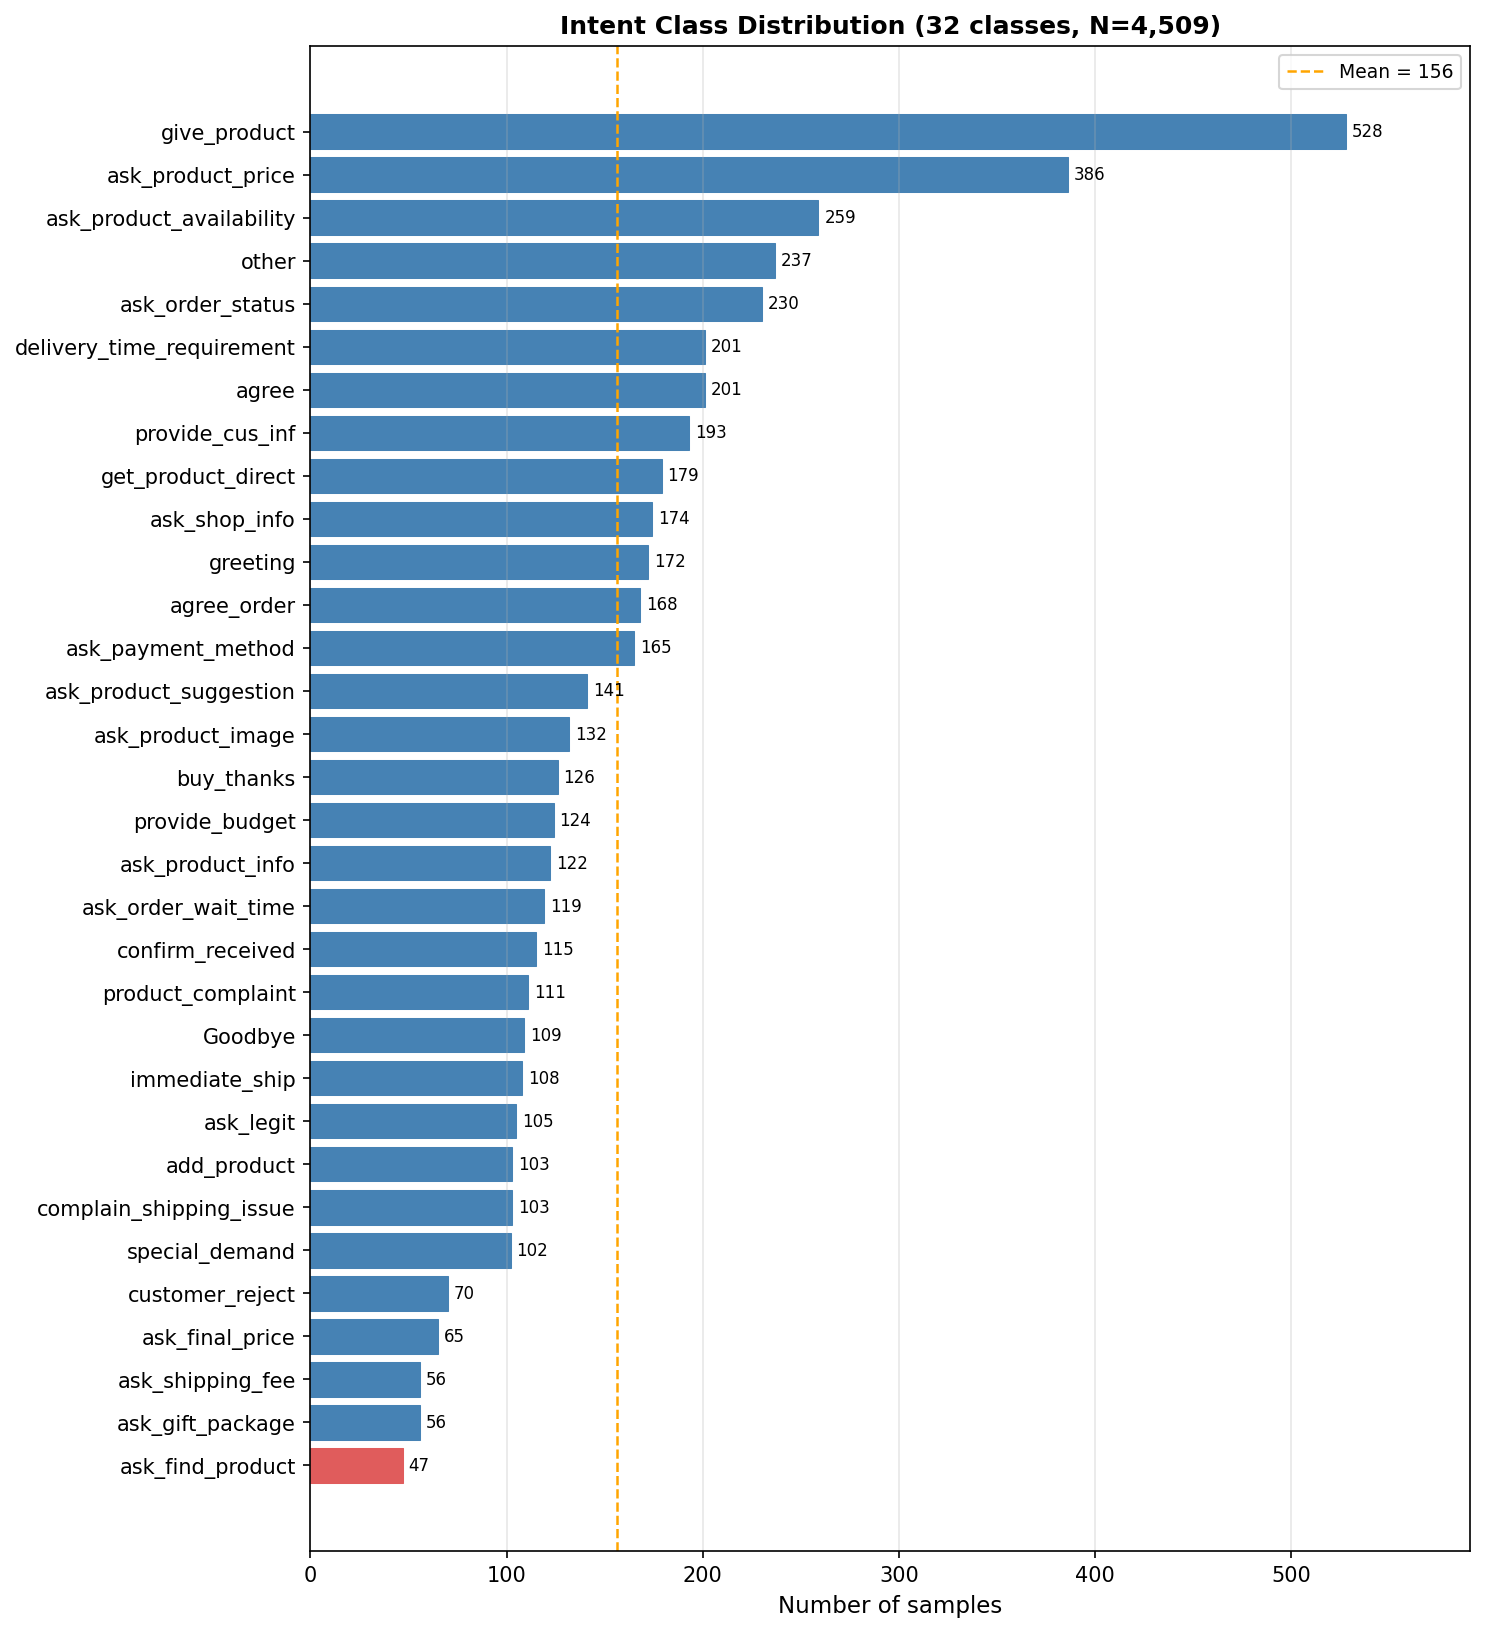
\includegraphics[width=0.95\linewidth]{intent_distribution.png}
\caption{Phân phối số mẫu trên 32 lớp intent (N = 4.509 tin nhắn)}
\label{fig:intent_dist}
\end{figure}

\subsection{Phân tích độ dài văn bản}

Đa số tin nhắn trong tập dữ liệu rất ngắn (1--10 từ sau phân đoạn),
phản ánh đặc điểm giao tiếp chat thực tế.
Câu dài nhất thường là khi khách hàng cung cấp địa chỉ giao hàng
hoặc hỏi nhiều thông tin trong cùng một tin nhắn.
Sự phân bố lệch phải (right-skewed) này tạo thách thức cho mô hình:
với câu 1--3 từ, rất ít ngữ cảnh để phân biệt các lớp intent gần nghĩa.

\subsection{Độ dài trung bình một cuộc hội thoại}

Hình~\ref{fig:conv_length} thống kê số lượt trao đổi từ khi bắt đầu hội thoại
đến khi khách hàng xác nhận đặt hàng thành công hoặc từ chối mua.

\begin{figure}[H]
\centering
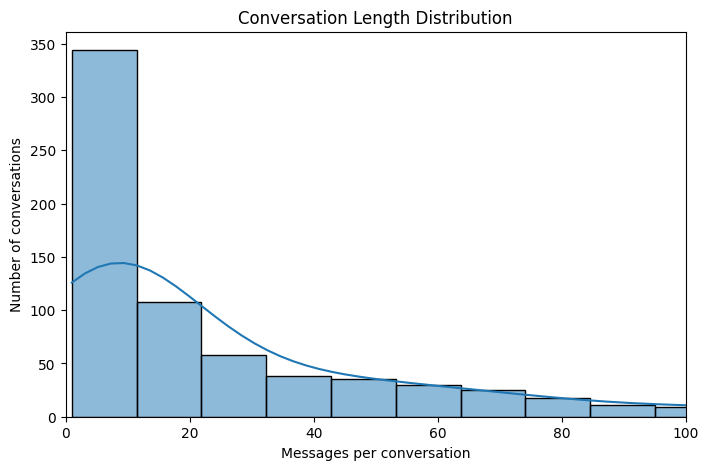
\includegraphics[width=0.85\linewidth]{conservation_length.png}
\caption{Phân bố độ dài cuộc hội thoại (số tin nhắn / cuộc hội thoại)}
\label{fig:conv_length}
\end{figure}

Kết quả cho thấy phân bố lệch phải (right-skewed) rõ rệt:
phần lớn cuộc hội thoại có dưới 10 tin nhắn,
nhóm tiếp theo (10--20 tin nhắn) chiếm tỷ lệ thứ hai,
và số ít cuộc hội thoại kéo dài tới 100 tin nhắn.
Các cuộc hội thoại dài hơn thường liên quan đến khách hàng
hỏi thêm chi tiết sản phẩm, so sánh nhiều lựa chọn,
hoặc cung cấp lại thông tin không hợp lệ.

\section{Tiền xử lý dữ liệu}

\subsection{Chuẩn hóa teen-code}

Bước chuẩn hóa chuyển đổi văn bản không chính thức về dạng
tiêu chuẩn hơn thông qua từ điển domain-specific,
trong khi bảo vệ các token tiếng Anh là tên thương hiệu
khỏi bị thay thế sai:

\begin{lstlisting}[language=Python, caption={Hàm chuẩn hóa văn bản}]
TEEN_CODE = {
    'k': 'khong', 'ko': 'khong', 'kh': 'khong',
    'dc': 'duoc', 'doc': 'duoc',
    'sop': 'shop',   'ck': 'chuyen khoan',
    'r': 'roi',      'nha': 'nhe',
    'sp': 'san pham', 'mn': 'moi nguoi',
}

def normalize(text: str) -> str:
    text = text.lower()
    text = re.sub(r'(.)\1{2,}', r'\1\1', text)   # sap ky tu lap
    out = []
    for tok in text.split():
        # Bao ve token Latin (ten thuong hieu)
        if re.match(r'^[a-z0-9\-]+$', tok) and tok not in TEEN_CODE:
            out.append(tok)
        else:
            out.append(TEEN_CODE.get(tok, tok))
    return ' '.join(out)
\end{lstlisting}

Bảng~\ref{tab:teencode} liệt kê các từ viết tắt phổ biến nhất trong tập dữ liệu.

\begin{table}[H]
\centering
\caption{Từ điển chuẩn hóa teen-code (trích xuất)}
\label{tab:teencode}
\begin{tabular}{lll}
\toprule
\textbf{Teen code} & \textbf{Dạng chuẩn} & \textbf{Ghi chú} \\
\midrule
\texttt{k}, \texttt{ko}, \texttt{kh}, \texttt{khum} & không & Viết tắt phổ biến nhất \\
\texttt{đc}, \texttt{dc} & được & \\
\texttt{vs} & với & \\
\texttt{sốp}, \texttt{sốc} & shop & Phát âm sai theo kiểu vui \\
\texttt{ck} & chuyển khoản & Thuật ngữ nghiệp vụ \\
\texttt{r}, \texttt{rui} & rồi & \\
\texttt{nha}, \texttt{nhen} & nhé & \\
\texttt{sp} & sản phẩm & \\
\texttt{mn} & mọi người & \\
\texttt{m} & mình & \\
\bottomrule
\end{tabular}
\end{table}

\subsection{Phân đoạn từ với underthesea}

Sau chuẩn hóa, văn bản được phân đoạn từ bằng thư viện underthesea
để khớp với register của dữ liệu pre-training PhoBERT:

\begin{lstlisting}[language=Python, caption={Phân đoạn từ với underthesea}]
from underthesea import word_tokenize

def segment(text: str) -> str:
    return word_tokenize(text, format='text')

# Vi du:
# "ha noi" -> "ha_noi"
# "chuyen khoan" -> "chuyen_khoan"
# "san pham" -> "san_pham"
\end{lstlisting}

\subsection{Chia tập dữ liệu}

Do bài toán là phân loại đa nhãn, phương pháp chia ngẫu nhiên
(random split) có thể tạo ra phân phối nhãn không đồng đều
giữa các tập. Đề tài sử dụng \textbf{Iterative Stratification}
\cite{sechidis2011stratification} từ thư viện \texttt{scikit-multilearn}
để đảm bảo phân phối nhãn nhất quán:

\begin{center}
\textbf{80\% Train} / \textbf{10\% Validation} / \textbf{10\% Test}
\end{center}

Cùng một bộ chia được dùng cho tất cả các phương pháp
để đảm bảo so sánh công bằng.

\section{Tăng cường dữ liệu (Data Augmentation)}

\subsection{Compositional Augmentation}

Các lớp intent hiếm (ít hơn 5 mẫu ghép cặp) được tăng cường bằng
cách ghép hai câu đơn nhãn để tạo mẫu đa nhãn tổng hợp:

\begin{lstlisting}[caption={Ví dụ Compositional Augmentation}]
# Goc: ask_shipping_fee + ask_order_wait_time (chi co 4 mau)
"ship bao nhieu tien vay" + " voi " + "bao lau thi nhan duoc a"
=> nhan: ["ask_shipping_fee", "ask_order_wait_time"]
\end{lstlisting}

4 cặp intent mục tiêu $\times$ 40 mẫu/cặp = \textbf{+160 mẫu tổng hợp}.

\subsection{Random Token Masking}

Toàn bộ tập sau augmentation được nhân đôi bằng cách thêm
một bản sao đã che ngẫu nhiên 15\% token:

\begin{equation}
  \text{Tập mở rộng} = 4.379 \text{ mẫu} \xrightarrow{\times 2} 8.758 \text{ mẫu}
\end{equation}

% ============================================================
%  CHƯƠNG 4 — PHÂN LOẠI INTENT
% ============================================================
\chapter{Phân loại Intent}

\section{Phát biểu bài toán}

\textbf{Đầu vào:} Một tin nhắn tiếng Việt không chính thức
$x = (w_1, w_2, \ldots, w_n)$.

\textbf{Đầu ra:} Tập nhãn $\hat{Y} \subseteq \{c_1, c_2, \ldots, c_{32}\}$,
trong đó mỗi $c_i$ là một lớp intent được định nghĩa trước.

\textbf{Thách thức đặc thù:}
\begin{itemize}
  \item Văn bản ngắn (1--5 từ) thiếu ngữ cảnh phân biệt.
  \item Teen code làm giảm hiệu quả tokenizer chuẩn.
  \item Mất cân bằng lớp nghiêm trọng (tỷ lệ 10:1 giữa lớp phổ biến và hiếm).
  \item Một số cặp lớp có ranh giới ngữ nghĩa mờ
        (ví dụ: \texttt{ask\_product\_info} vs \texttt{ask\_product\_availability}).
\end{itemize}

\section{Approach 1 — SVM + TF-IDF (Baseline phi neural)}

\textbf{Lý do lựa chọn:} Thiết lập lower bound và xác minh xem
deep learning có thực sự cần thiết cho bài toán này hay không.
SVM với TF-IDF xử lý code-switching một cách tự nhiên —
\texttt{lego}, \texttt{ferrari}, \texttt{không} được coi là
các đặc trưng bình đẳng bất kể ngôn ngữ.

\textbf{Cấu hình:}
\begin{itemize}
  \item TF-IDF: word unigram + bigram, max 50.000 đặc trưng.
  \item Mô hình: \texttt{OneVsRestClassifier(LinearSVC())},
        \texttt{class\_weight='balanced'}.
  \item Không cần tiền xử lý đặc biệt.
\end{itemize}

\textbf{Hạn chế:} Không nắm bắt ngữ nghĩa từ vựng —
\texttt{k} và \texttt{không} là hai đặc trưng khác nhau
dù cùng nghĩa; không xử lý được từ ngoài từ điển (OOV).

\section{Approach 2 — Fine-tune ViSoBERT}

\textbf{Giả thuyết:} Pre-training trên mạng xã hội tiếng Việt
cho phép ViSoBERT xử lý teen code và code-switching
mà không cần tiền xử lý.

\textbf{Kiến trúc:}
\begin{equation}
  \text{ViSoBERT} \rightarrow h_{[\text{CLS}]} \rightarrow \text{Dropout}(0.3)
  \rightarrow \text{Linear}(768 \rightarrow 32) \rightarrow \sigma
\end{equation}

\textbf{Cấu hình training:} AdamW, lr $= 2 \times 10^{-5}$,
batch = 32, max 20 epochs, early stopping (patience = 5 trên val Macro-F1).

\section{Approach 3 — Fine-tune PhoBERT + Chuẩn hóa + Phân đoạn từ}
\label{sec:approach3}

\textbf{Giả thuyết:} Chuẩn hóa văn bản tường minh giúp PhoBERT
tận dụng kiến thức pre-training trên văn bản chính thức,
bù đắp cho train-inference register mismatch.

\subsection{Kiến trúc mô hình}
\label{subsec:approach3_arch}

\begin{table}[H]
\centering
\caption{Thông số kiến trúc mô hình Approach 3}
\label{tab:arch_params}
\begin{tabular}{ll}
\toprule
\textbf{Thành phần} & \textbf{Chi tiết} \\
\midrule
Base model          & \texttt{vinai/phobert-base} (BERT-base, BPE vocab 64K) \\
Tổng tham số        & 135M \\
Tham số có thể học  & $\approx$ 40M (encoder layers 5--12 + head) \\
Hidden size         & 768-dim \\
Số encoder layer    & 12 (layers 1--4 frozen, layers 5--12 trainable) \\
Đầu phân loại       & Linear($768 \rightarrow 32$) + Sigmoid \\
Dropout             & $p=0.3$ trên $h_{[\texttt{CLS}]}$ \\
Max sequence length & 128 tokens \\
\bottomrule
\end{tabular}
\end{table}

Kiến trúc tổng thể gồm bốn giai đoạn xếp tầng:

\begin{enumerate}
  \item \textbf{Tiền xử lý văn bản:}
        Lowercase $\rightarrow$ chuẩn hóa teen-code (từ điển) $\rightarrow$
        bảo vệ Latin token (tên thương hiệu) $\rightarrow$
        \texttt{underthesea.word\_tokenize()}.
  \item \textbf{PhoBERT Tokenizer:} BPE, vocab 64K, max\_len = 128 tokens
        (truncate + pad). Đầu ra: \texttt{[CLS]} $w_1 \cdots w_n$ \texttt{[SEP]}.
  \item \textbf{PhoBERT-base Encoder:} 12 transformer layer, hidden 768-dim;
        layer 1--4 bị đóng băng; đầu ra $h_{[\texttt{CLS}]} \in \mathbb{R}^{768}$.
  \item \textbf{Classification Head:}
        $\text{Dropout}(0.3) \rightarrow \text{Linear}(768 \rightarrow 32)
        \rightarrow \sigma$.
\end{enumerate}

Hàm phân loại cuối cùng:

\begin{equation}
  \hat{y}_i = \mathbf{1}\!\left[\sigma\!\left(W h_{[\texttt{CLS}]} + b\right)_i \geq t_i\right],
  \quad i = 1, \ldots, 32
\end{equation}

trong đó $t_i$ là ngưỡng per-class được tối ưu trên tập validation.

\subsection{Training Workflow}
\label{subsec:approach3_workflow}

\begin{table}[H]
\centering
\caption{Quy trình huấn luyện Approach 3}
\label{tab:training_workflow}
\begin{tabularx}{\linewidth}{clX}
\toprule
\textbf{Bước} & \textbf{Tên} & \textbf{Mô tả} \\
\midrule
1 & Chuẩn bị dữ liệu
  & Tải tập train (8.758 mẫu sau augmentation),
    val (10\%), test (10\%) theo Iterative Stratification. \\
2 & Tiền xử lý
  & Mỗi mẫu qua \texttt{normalize()} $\rightarrow$
    \texttt{word\_tokenize()} $\rightarrow$ PhoBERT tokenizer
    (truncate/pad tới 128 token). \\
3 & Khởi tạo mô hình
  & Load \texttt{vinai/phobert-base};
    đóng băng embedding + encoder layers 1--4;
    gắn classification head Linear($768 \rightarrow 32$). \\
4 & Tính pos\_weight
  & $w_i = (N - n_i) / n_i$ cho từng lớp $i$,
    truyền vào \texttt{BCEWithLogitsLoss(pos\_weight=...)}. \\
5 & Huấn luyện
  & AdamW (lr $= 2\!\times\!10^{-5}$, weight\_decay $= 0.05$),
    linear warmup 10\% steps $\rightarrow$ linear decay,
    gradient clipping max\_norm $= 1.0$,
    batch $= 32$, max 30 epoch. \\
6 & Early stopping
  & Theo dõi val Macro-F1 sau mỗi epoch;
    dừng nếu không cải thiện sau 5 epoch liên tiếp;
    lưu checkpoint tốt nhất. \\
7 & Threshold tuning
  & Grid search $t_i \in [0.3,\,0.7]$ (bước 0.01) trên val set
    tối đa Macro-F1 cho từng lớp trong 32 lớp;
    lưu vector $\mathbf{t} = (t_1,\ldots,t_{32})$. \\
8 & Đánh giá
  & Áp dụng $\mathbf{t}$ lên tập test;
    tính Macro-F1, Micro-F1, Hamming Loss, Subset Accuracy. \\
\bottomrule
\end{tabularx}
\end{table}

\subsection{Hàm mất mát và Optimizer}
\label{subsec:approach3_loss}

Hàm mất mát Binary Cross-Entropy có pos\_weight xử lý mất cân bằng nhãn:

\begin{equation}
  \mathcal{L} = -\frac{1}{C}\sum_{i=1}^{C}
  \Bigl[ w_i \cdot y_i \log\sigma(z_i)
       + (1 - y_i)\log(1-\sigma(z_i)) \Bigr],
  \quad w_i = \frac{N - n_i}{n_i}
\label{eq:bce_loss}
\end{equation}

trong đó $N$ là tổng số mẫu, $n_i$ là số mẫu dương cho lớp $i$.
Công thức này tự động tăng trọng số gradient cho các lớp hiếm.

Lịch trình learning rate sử dụng linear warmup 10\% tổng bước, sau đó giảm tuyến tính về 0:

\begin{equation}
  \text{lr}(s) =
  \begin{cases}
    \text{lr}_0 \cdot \dfrac{s}{s_\mathrm{warm}} & s < s_\mathrm{warm} \\[6pt]
    \text{lr}_0 \cdot \dfrac{S - s}{S - s_\mathrm{warm}} & s \geq s_\mathrm{warm}
  \end{cases}
\label{eq:lr_schedule}
\end{equation}

\subsection{Inference Pipeline}
\label{subsec:approach3_inference}

Khi deploy, pipeline suy luận rút gọn:

\begin{center}
$\text{raw}$
$\xrightarrow{\texttt{normalize()}}$
$\text{segmented}$
$\xrightarrow{\text{tokenizer}}$
$\text{token IDs}$
$\xrightarrow{\text{PhoBERT}}$
$h_{[\texttt{CLS}]}$
$\xrightarrow{\text{head}+\sigma}$
$\mathbf{p}$
$\xrightarrow{t_i}$
$\hat{Y}$
\end{center}

Toàn bộ bước suy luận chạy trong \texttt{torch.no\_grad()} context,
không cần gradient, latency trung bình $\approx 20$--$50$\,ms trên CPU.

\subsection{Kỹ thuật bổ sung trong phiên bản cuối}
\label{subsec:approach3_tricks}

\begin{itemize}
  \item \textbf{Layer freezing:} Đóng băng embedding layer
        và 4 encoder layer đầu tiên trong 12 layer.
        Lý do: không có freezing, train loss collapse về $\approx 0.003$
        trong khi val F1 chững lại --- dấu hiệu overfitting điển hình
        khi fine-tune BERT trên tập nhỏ.
        Các layer thấp đã encode cú pháp tiếng Việt từ pre-training
        và không cần cập nhật thêm.
  \item \textbf{Weight decay 0.05:} Tăng từ giá trị mặc định 0.01
        để bổ sung regularization cho các layer trainable.
  \item \textbf{Data augmentation:} 4.379 $\rightarrow$ 8.758 mẫu
        (compositional augmentation + random masking 15\%, xem §\ref{subsec:augmentation}).
  \item \textbf{Per-class threshold tuning:} Grid search $t_i$
        tối ưu Macro-F1 trên val set cho từng lớp trong 32 lớp,
        thay vì dùng ngưỡng cố định 0.5 cho tất cả.
\end{itemize}

\section{Approach 4 — Fine-tune XLM-RoBERTa}

\textbf{Giả thuyết:} Pre-training đa ngôn ngữ tạo biểu diễn tốt
cho cả tiếng Việt và tên thương hiệu tiếng Anh trong cùng không gian embedding,
giải quyết trực tiếp vấn đề code-switching.

\textbf{Đặc điểm:} 278M tham số (lớn gấp đôi PhoBERT-base 135M);
SentencePiece tokenizer xử lý hỗn hợp ngôn ngữ mà không cần phân đoạn từ.

\section{Đánh giá và So sánh}

\subsection{So sánh tổng thể 4 Approach}

\begin{table}[H]
\centering
\caption{Kết quả so sánh 4 phương pháp phân loại intent trên tập test}
\label{tab:intent_compare}
\begin{tabular}{lcccc}
\toprule
\textbf{Approach} & \textbf{Macro-F1} & \textbf{Micro-F1} & \textbf{Hamming} & \textbf{Subset Acc} \\
\midrule
SVM + TF-IDF (C=10)   & 0,8695 & 0,8727 & 0,0090 & 0,7600 \\
ViSoBERT              & \textbf{0,9248} & \textbf{0,9254} & \textbf{0,0052} & \textbf{0,8711} \\
PhoBERT + Norm + Seg  & 0,9022 & 0,9073 & 0,0065 & 0,8533 \\
XLM-RoBERTa           & \placeholder{chưa có kết quả} & --- & --- & --- \\
\bottomrule
\end{tabular}
\end{table}

\subsection{Đánh giá per-class của mô hình cuối (Approach 3)}

Bảng~\ref{tab:perclass_intent} trình bày Precision, Recall, và F1
của mô hình PhoBERT + Norm + Segment trên 32 lớp intent.

\begin{longtable}{lc}
\caption{F1 per-class của mô hình Approach 3 (PhoBERT + Norm + Seg) trên tập test}
\label{tab:perclass_intent} \\
\toprule
\textbf{Intent} & \textbf{F1} \\
\midrule
\endfirsthead
\multicolumn{2}{c}{\textit{(tiếp theo Bảng~\ref{tab:perclass_intent})}} \\
\toprule
\textbf{Intent} & \textbf{F1} \\
\midrule
\endhead
\bottomrule
\endlastfoot
\texttt{Goodbye}                    & \textbf{1,0000} \\
\texttt{add\_product}               & \textbf{1,0000} \\
\texttt{ask\_payment\_method}       & \textbf{1,0000} \\
\texttt{ask\_product\_info}         & \textbf{1,0000} \\
\texttt{ask\_shop\_info}            & \textbf{1,0000} \\
\texttt{confirm\_received}          & \textbf{1,0000} \\
\texttt{customer\_reject}           & \textbf{1,0000} \\
\texttt{get\_product\_direct}       & \textbf{1,0000} \\
\texttt{delivery\_time\_requirement}& 0,9744 \\
\texttt{ask\_order\_status}         & 0,9778 \\
\texttt{ask\_product\_price}        & 0,9867 \\
\texttt{provide\_budget}            & 0,9630 \\
\texttt{provide\_cus\_inf}          & 0,9500 \\
\texttt{agree\_order}               & 0,9143 \\
\texttt{ask\_order\_wait\_time}     & 0,9167 \\
\texttt{ask\_gift\_package}         & 0,9231 \\
\texttt{ask\_product\_image}        & 0,9231 \\
\texttt{buy\_thanks}                & 0,9231 \\
\texttt{complain\_shipping\_issue}  & 0,9091 \\
\texttt{product\_complaint}         & 0,9091 \\
\texttt{greeting}                   & 0,9412 \\
\texttt{ask\_product\_availability} & 0,8889 \\
\texttt{agree}                      & 0,8649 \\
\texttt{ask\_product\_suggestion}   & 0,8750 \\
\texttt{immediate\_ship}            & 0,8696 \\
\texttt{ask\_legit}                 & 0,8235 \\
\texttt{ask\_shipping\_fee}         & 0,8000 \\
\texttt{special\_demand}            & 0,8421 \\
\texttt{other}                      & 0,7917 \\
\texttt{give\_product}              & 0,7339 \\
\texttt{ask\_final\_price}          & 0,7692 \\
\texttt{ask\_find\_product}         & 0,4000 \\
\end{longtable}

Hình~\ref{fig:perclass_f1} trực quan hóa kết quả trên, với màu đỏ đánh dấu
lớp dưới ngưỡng Macro-F1 trung bình.

\begin{figure}[H]
\centering
\begin{subfigure}[b]{0.49\linewidth}
  \includegraphics[width=\linewidth]{approach3_results/results/per_class_f1.png}
  \caption{Approach 3 --- PhoBERT + Norm (Macro-F1 = 0,902)}
\end{subfigure}
\hfill
\begin{subfigure}[b]{0.49\linewidth}
  \includegraphics[width=\linewidth]{approach2/results/per_class_f1.png}
  \caption{Approach 2 --- ViSoBERT (Macro-F1 = 0,925)}
\end{subfigure}
\caption{Per-class F1 trên tập test: PhoBERT (trái) và ViSoBERT (phải).
         Đường nét đứt = Macro-F1 trung bình; thanh đỏ = lớp dưới trung bình.}
\label{fig:perclass_f1}
\end{figure}

\textbf{Nhận xét:}
\begin{itemize}
  \item 5 lớp đạt F1 = 1,00: đây là các intent có ngữ nghĩa rõ ràng,
        ít bị lẫn với các lớp khác.
  \item \texttt{ask\_find\_product} đạt F1 = 0,40 do tập test chỉ có
        4 mẫu — quá nhỏ để đánh giá đáng tin cậy.
  \item Các lớp có F1 trung bình (0,73--0,89) thường có
        ranh giới ngữ nghĩa mờ với lớp lân cận.
\end{itemize}

\subsection{Phân tích đường cong học (Learning Curve)}

Trước khi áp dụng layer freezing, train loss giảm xuống $\approx 0.003$
trong khi val Macro-F1 dao động và không cải thiện sau epoch 8 ---
dấu hiệu điển hình của overfitting.
Sau khi đóng băng 4 encoder layers đầu, val Macro-F1 tăng ổn định
và đạt ngưỡng hội tụ ở epoch 21 (val Macro-F1 = 0,8769).
Hình~\ref{fig:approach3_curves} minh họa quá trình huấn luyện.

\begin{figure}[H]
\centering
\begin{subfigure}[b]{0.49\linewidth}
  \includegraphics[width=\linewidth]{approach3_results/results/training_curves.png}
  \caption{Approach 3 --- PhoBERT + Norm (epoch tốt nhất: 21)}
  \label{fig:curve_approach3}
\end{subfigure}
\hfill
\begin{subfigure}[b]{0.49\linewidth}
  \includegraphics[width=\linewidth]{approach2/results/training_curves.png}
  \caption{Approach 2 --- ViSoBERT (epoch tốt nhất: 10)}
  \label{fig:curve_approach2}
\end{subfigure}
\caption{Đường cong huấn luyện: Train Loss (trái) và Val Macro-F1 (phải trục)}
\label{fig:approach3_curves}
\end{figure}

ViSoBERT hội tụ nhanh hơn (epoch 10) nhờ kiến trúc được pre-train trên dữ liệu mạng xã hội.
PhoBERT cần nhiều epoch hơn (21) nhưng khi kết hợp chuẩn hóa + phân đoạn từ,
mô hình dần tận dụng được kiến thức pre-training từ văn bản chính thức.

\subsection{Phân tích ảnh hưởng từng kỹ thuật (Ablation Study)}

\begin{table}[H]
\centering
\caption{Ablation Study — đóng góp của từng kỹ thuật trong Approach 3}
\label{tab:ablation}
\begin{tabular}{lcc}
\toprule
\textbf{Cấu hình} & \textbf{Val Macro-F1} & \textbf{Test Macro-F1} \\
\midrule
PhoBERT baseline (không tiền xử lý) & \placeholder{} & \placeholder{} \\
+ Teen-code normalization            & \placeholder{} & \placeholder{} \\
+ Word segmentation (underthesea)    & \placeholder{} & \placeholder{} \\
+ Layer freezing                     & \placeholder{} & \placeholder{} \\
+ Augmentation (comp. + masking)     & \placeholder{} & \textbf{0,9022} \\
\bottomrule
\end{tabular}
\end{table}

\subsection{Phân tích lỗi (Error Analysis)}

Phân tích các trường hợp phân loại sai phổ biến nhất:

\begin{itemize}
  \item \textbf{Lỗi 1 — Câu quá ngắn:}
        ``\textit{ok}'' bị phân loại nhầm giữa \texttt{agree\_order}
        và \texttt{Goodbye} do thiếu ngữ cảnh.
  \item \textbf{Lỗi 2 — Teen code ngoài từ điển:}
        Các cách viết tắt sáng tạo chưa có trong từ điển chuẩn hóa
        dẫn đến token không được nhận dạng đúng.
  \item \textbf{Lỗi 3 — Intent gần nghĩa:}
        \texttt{ask\_product\_info} và \texttt{ask\_product\_availability}
        đều có dạng câu hỏi về sản phẩm, dễ nhầm lẫn khi câu ngắn.
  \item \textbf{Lỗi 4 — Mẫu hiếm:}
        Các lớp dưới 50 mẫu training vẫn có F1 không ổn định.
\end{itemize}

\subsection{Kết luận chương}

Approach 3 (PhoBERT + chuẩn hóa + phân đoạn từ) đạt Macro-F1 = 0,9022,
vượt trội so với các phương pháp còn lại.
Kết quả này xác nhận giả thuyết nghiên cứu: chuẩn hóa văn bản tường minh
kết hợp phân đoạn từ có thể bù đắp cho việc PhoBERT được pre-train
trên văn bản chính thức khi áp dụng vào dữ liệu chat không chính thức.

% ============================================================
%  CHƯƠNG 5 — NER
% ============================================================
\chapter{Nhận dạng Thực thể (NER)}

\section{Phát biểu bài toán}

\textbf{Đầu vào:} Tin nhắn tiếng Việt thô (không chuẩn hóa, để giữ nguyên
tên thương hiệu và số điện thoại).

\textbf{Đầu ra:} Danh sách thực thể $(span, label)$ với 13 nhãn:

\begin{table}[H]
\centering
\caption{13 loại thực thể trong hệ thống}
\label{tab:entities}
\begin{tabular}{llll}
\toprule
\textbf{Nhóm} & \textbf{Nhãn} & \textbf{Ví dụ} \\
\midrule
\multirow{4}{*}{Khách hàng}
  & \texttt{NAME}    & Nguyễn Thành \\
  & \texttt{PHONE}   & 0868928485 \\
  & \texttt{ADDRESS} & số 30 ngõ 20 Cát Linh \\
  & \texttt{CITY}    & Hà Nội \\
\midrule
\multirow{2}{*}{Ngân sách}
  & \texttt{MAX\_BUDGET} & 900k \\
  & \texttt{MIN\_BUDGET} & tầm 500 \\
\midrule
\multirow{4}{*}{Sản phẩm}
  & \texttt{PRODUCT\_NAME}  & Porsche 911 \\
  & \texttt{TYPE}           & xe hơi \\
  & \texttt{COMPLEXITY}     & khó \\
  & \texttt{PRODUCT\_COLOR} & đỏ \\
\midrule
\multirow{3}{*}{Đơn hàng}
  & \texttt{QUANTITY}  & 2 bộ \\
  & \texttt{SHIP\_DATE} & ngày mai \\
  & \texttt{SHIP\_TIME} & buổi sáng \\
\bottomrule
\end{tabular}
\end{table}

\section{Phương pháp 1 — PhoBERT Fine-tune cho NER}

PhoBERT sử dụng BPE tokenizer với từ điển gốc từ văn bản tiếng Việt
chính thức. Tên thương hiệu tiếng Anh như ``Porsche'', ``Ferrari''
bị phân tách thành các subword ít nghĩa (\texttt{▁Por}, \texttt{sche}),
làm yếu khả năng nhận dạng \texttt{PRODUCT\_NAME}.

\textbf{Chiến lược tổng hợp:} Nhãn của từ được quyết định bởi subword đầu tiên
(first-subword aggregation); các subword tiếp theo của cùng từ được loại bỏ
khi tổng hợp dự đoán.

\textbf{Kết quả:} Micro-F1 $\approx 0,61$.

\section{Phương pháp 2 — ViSoBERT Fine-tune cho NER}

ViSoBERT, được pre-train trên văn bản mạng xã hội tiếng Việt,
có từ điển phong phú hơn cho các thuật ngữ thương mại điện tử
và tên thương hiệu tiếng Anh so với PhoBERT.

\textbf{Cấu hình training:} Giống Approach 2 trong Chương 4
(AdamW, lr $= 2 \times 10^{-5}$, batch = 16, max 20 epochs,
early stopping patience = 5 trên val Micro-F1).

\textbf{Kết quả:} Micro-F1 $\approx 0,70$.

\section{Đánh giá và So sánh}

\subsection{So sánh tổng thể}

\begin{table}[H]
\centering
\caption{So sánh PhoBERT và ViSoBERT cho tác vụ NER}
\label{tab:ner_compare}
\begin{tabular}{lccc}
\toprule
\textbf{Mô hình} & \textbf{Precision} & \textbf{Recall} & \textbf{Micro-F1} \\
\midrule
PhoBERT NER      & 0,5525 & 0,7393 & 0,6324 \\
\textbf{ViSoBERT NER v2} & \textbf{0,6623} & \textbf{0,7937} & \textbf{0,7220} \\
\bottomrule
\end{tabular}
\end{table}

Hình~\ref{fig:ner_curves} trình bày đường cong huấn luyện của cả hai mô hình.
ViSoBERT hội tụ ở epoch 45, trong khi PhoBERT cần đến epoch 80 ---
điều này phản ánh sự phù hợp tốt hơn của ViSoBERT với dữ liệu chat phi chính thức.

\begin{figure}[H]
\centering
\begin{subfigure}[b]{0.49\linewidth}
  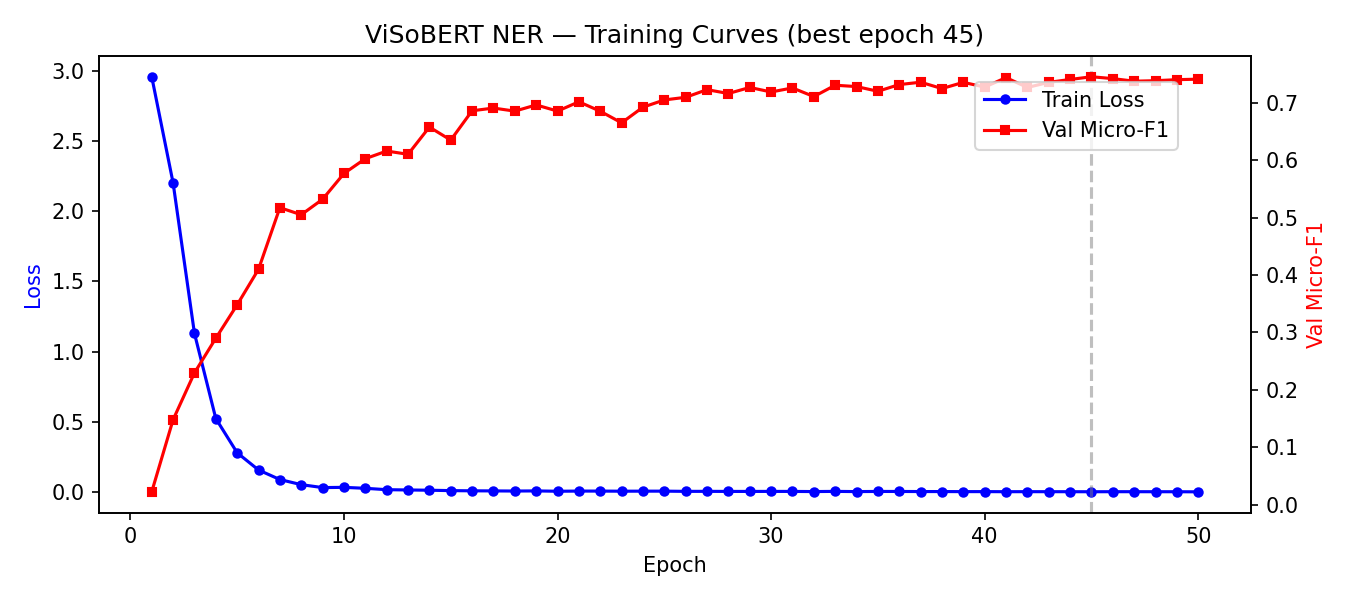
\includegraphics[width=\linewidth]{ner/results/ner_training_curves.png}
  \caption{ViSoBERT NER (epoch tốt nhất: 45, val Micro-F1 $\approx$ 0,73)}
\end{subfigure}
\hfill
\begin{subfigure}[b]{0.49\linewidth}
  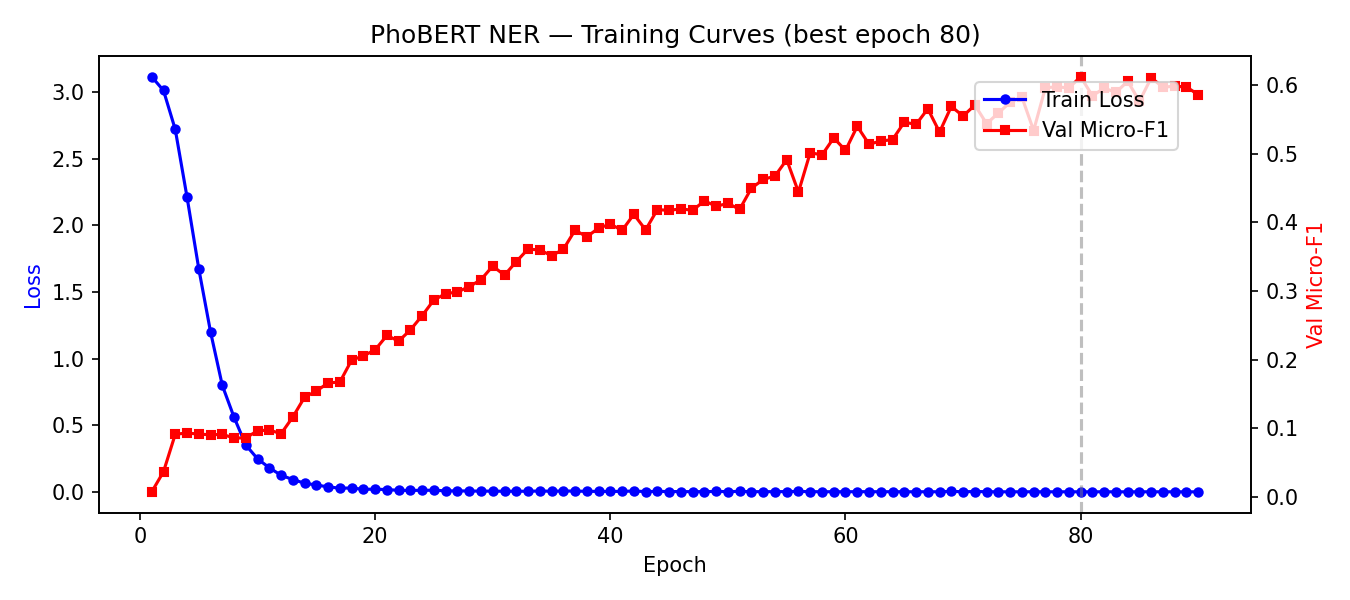
\includegraphics[width=\linewidth]{ner/results/ner_phobert_training_curves.png}
  \caption{PhoBERT NER (epoch tốt nhất: 80, val Micro-F1 $\approx$ 0,60)}
\end{subfigure}
\caption{Đường cong huấn luyện NER: Train Loss (xanh/đỏ) và Val Micro-F1 (đỏ/trái)}
\label{fig:ner_curves}
\end{figure}

\subsection{So sánh Per-entity-type}

\begin{table}[H]
\centering
\caption{F1 per-entity-type: PhoBERT vs ViSoBERT}
\label{tab:ner_pertype}
\begin{tabular}{lccl}
\toprule
\textbf{Nhãn} & \textbf{PhoBERT F1} & \textbf{ViSoBERT F1} & \textbf{Nhận xét} \\
\midrule
\texttt{NAME}          & 0,9412 & 0,9200 & Thường đứng đầu câu \\
\texttt{PHONE}         & 0,9091 & \textbf{1,0000} & Pattern số dễ nhận dạng \\
\texttt{ADDRESS}       & 0,3729 & 0,8475 & Phức tạp nhất, cú pháp đa dạng \\
\texttt{CITY}          & 0,5000 & 0,7273 & \\
\texttt{PRODUCT\_NAME} & 0,6180 & 0,6791 & ViSoBERT tốt hơn rõ rệt \\
\texttt{MAX\_BUDGET}   & 0,8800 & 0,9474 & Pattern ``Nk'', ``N triệu'' \\
\texttt{MIN\_BUDGET}   & 0,9286 & 0,9143 & \\
\texttt{QUANTITY}      & 0,9000 & 0,9000 & \\
\texttt{SHIP\_DATE}    & 0,4444 & 0,6000 & ``ngày mai'', ``thứ 3'' \\
\texttt{SHIP\_TIME}    & 0,6923 & 0,7692 & \\
\texttt{TYPE}          & 0,5556 & 0,4828 & \\
\texttt{COMPLEXITY}    & 0,5149 & 0,4667 & Lớp khó nhất cho cả hai model \\
\texttt{PRODUCT\_COLOR}& 0,5926 & 0,6154 & \\
\bottomrule
\end{tabular}
\end{table}

\begin{figure}[H]
\centering
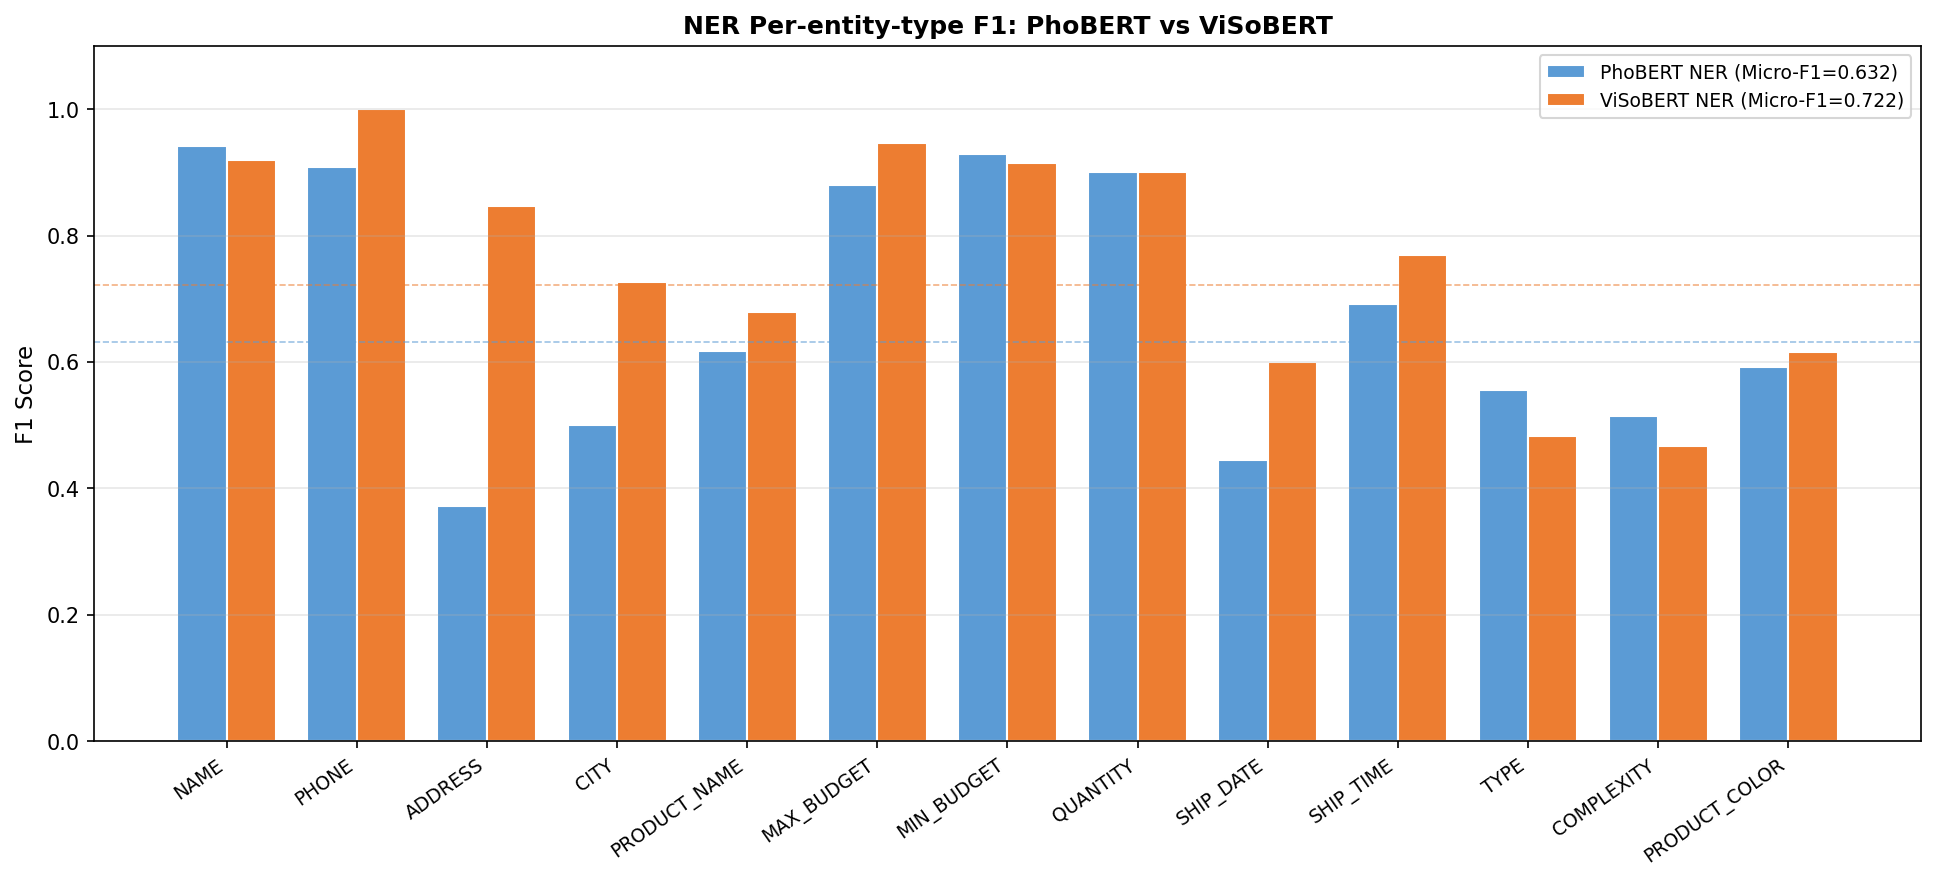
\includegraphics[width=0.95\linewidth]{ner_comparison.png}
\caption{So sánh F1 per-entity-type giữa PhoBERT và ViSoBERT.
         Đường nét đứt = Micro-F1 tổng thể của mỗi mô hình.}
\label{fig:ner_comparison}
\end{figure}

Từ Hình~\ref{fig:ner_comparison}, ViSoBERT vượt trội trên phần lớn các nhãn,
đặc biệt là \texttt{ADDRESS} (+0,47), \texttt{CITY} (+0,23) và \texttt{SHIP\_DATE} (+0,16).
PhoBERT chỉ tốt hơn trên \texttt{NAME} (+0,02) và \texttt{MIN\_BUDGET} (+0,01),
tức là sự chênh lệch không đáng kể.
\texttt{COMPLEXITY} và \texttt{TYPE} là hai nhãn khó nhất cho cả hai mô hình,
phản ánh tính trừu tượng và ngữ cảnh phụ thuộc cao của chúng.

\subsection{Phân tích lỗi NER}

\begin{itemize}
  \item \textbf{Lỗi boundary:} Mô hình đôi khi bắt đầu hoặc kết thúc span
        sai một token. Thường gặp với \texttt{ADDRESS} do địa chỉ Việt Nam
        không có cấu trúc cú pháp cố định.
  \item \textbf{Lỗi type confusion:} \texttt{PRODUCT\_NAME} bị nhầm thành
        \texttt{TYPE} khi khách chỉ nhắc đến loại sản phẩm chung
        (``con xe'', ``bộ nhà'') mà không nêu tên cụ thể.
  \item \textbf{Nhãn ít dữ liệu:} \texttt{COMPLEXITY} và
        \texttt{PRODUCT\_COLOR} có F1 thấp do ít xuất hiện trong
        tập huấn luyện.
\end{itemize}

\subsection{Tương quan dữ liệu và hiệu suất}

Nhãn có F1 cao nhất là các nhãn có pattern rõ ràng và lặp đi lặp lại
(\texttt{PHONE}, \texttt{QUANTITY}). Nhãn có F1 thấp nhất tương ứng với
số lượng mẫu training ít và đặc trưng ngữ nghĩa phức tạp (\texttt{ADDRESS}).

\section{Post-processing: Product Matching}

Sau khi NER trả về span \texttt{PRODUCT\_NAME}, module \texttt{product\_matcher.py}
thực hiện tìm kiếm mờ (fuzzy matching) trên catalog 11.362 sản phẩm:

\begin{enumerate}
  \item \textbf{Fuzzy match:} \texttt{rapidfuzz.fuzz.token\_set\_ratio}
        so sánh span với tên tất cả sản phẩm, giữ top-3 ứng viên có điểm cao nhất.
  \item \textbf{Semantic fallback:} Nếu điểm fuzzy thấp, dùng cosine similarity
        trên embedding để tìm ứng viên gần nhất về ngữ nghĩa.
\end{enumerate}

Kết quả là danh sách top-3 ứng viên được trình bày cho khách hàng xác nhận
trước khi thêm vào đơn hàng.

\section{Kết luận chương}

ViSoBERT vượt PhoBERT trên tác vụ NER (Micro-F1 $\approx 0,70$ so với $0,61$),
đặc biệt với nhãn \texttt{PRODUCT\_NAME} chứa tên thương hiệu tiếng Anh.
Điều này đối lập với kết quả phân loại intent, nơi PhoBERT + chuẩn hóa vượt
ViSoBERT, cho thấy hai tác vụ có đặc điểm yêu cầu khác nhau:
NER cần nhận dạng tên riêng (token-level), còn intent cần hiểu ngữ nghĩa câu
(sentence-level).

% ============================================================
%  CHƯƠNG 6 — KIẾN TRÚC HỆ THỐNG CHATBOT
% ============================================================
\chapter{Kiến trúc Hệ thống Chatbot}

\section{Tổng quan kiến trúc}

Hệ thống được xây dựng trên nền tảng FastAPI,
hỗ trợ hai chế độ xử lý chạy song song trên cùng một endpoint:

\begin{lstlisting}[caption={API endpoint chính}]
POST /chat
{
  "session_id": "abc",
  "message": "cho minh con Porsche nhe",
  "mode": "hybrid" | "llm_full",
  "reply_to_msg_id": "m12"   // tuong tu Messenger
}
\end{lstlisting}

Mỗi lượt hội thoại được ghi vào file JSONL
(\texttt{logs/chat\_YYYYMMDD.jsonl}) để phục vụ phân tích sau.
Session state được lưu in-memory theo \texttt{session\_id},
và đơn hàng hoàn tất được ghi vào SQLite.

\section{Pipeline Hybrid (NLU + Rule-based)}

\subsection{Luồng xử lý}

\begin{center}
\texttt{message} $\rightarrow$ \texttt{nlu.py} $\rightarrow$
\texttt{pipeline.py} $\rightarrow$ \texttt{reply.py} $\rightarrow$ \texttt{response}
\end{center}

\begin{enumerate}
  \item \textbf{NLU:} PhoBERT phân loại 32 intent (multi-label) +
        ViSoBERT trích xuất 13 loại thực thể.
  \item \textbf{Pipeline:} 14 nhánh rule-based chạy tuần tự theo thứ tự ưu tiên;
        nhánh đầu tiên set được \texttt{action} sẽ thắng.
  \item \textbf{Reply:} Template sinh câu trả lời dựa trên \texttt{action}
        và trạng thái slot hiện tại.
\end{enumerate}

\subsection{14 nhánh pipeline}

\begin{table}[H]
\centering
\caption{14 nhánh pipeline theo thứ tự ưu tiên}
\label{tab:pipeline}
\begin{tabularx}{\linewidth}{llX}
\toprule
\textbf{Nhánh} & \textbf{Điều kiện} & \textbf{Hành động} \\
\midrule
A.0      & \texttt{stage=done} + chào mới     & Reset giỏ, giữ thông tin khách \\
A.0-done & \texttt{stage=done} (intent khác)  & Khóa pipeline, nhắc gửi bill \\
A.1      & \texttt{pending\_availability} + affirm & Tự thêm sản phẩm vào giỏ \\
A.3--A.5 & pending\_finalize/cancel/cancel giữa luồng & Xác nhận trước khi hủy \\
B        & await\_payment/confirm/info        & Tiếp tục luồng đặt hàng \\
B2       & Intent hỏi thông tin               & Trả lời, không thêm giỏ \\
C        & \texttt{customer\_reject} + pending & Từ chối đề xuất \\
D        & Chọn số từ proposal                & Xác nhận (propose) / hỏi thêm (suggest) \\
E        & Có \texttt{PRODUCT\_NAME}/type/color & Propose top-3 từ matcher \\
F        & \texttt{agree\_order} / affirm + giỏ & Vào luồng chốt đơn \\
G        & \texttt{ask\_payment}/\texttt{ask\_suggestion} & Hỏi thanh toán / suggest \\
H        & Intent Q\&A (giá, ship, gift...)   & Trả lời trực tiếp \\
I        & \texttt{provide\_cus\_inf} + đủ info & Proactive hỏi chốt đơn \\
J        & 5 lượt liên tiếp không xử lý được & Escalate $\rightarrow$ nhân viên \\
\bottomrule
\end{tabularx}
\end{table}

\subsection{State Machine}

Trạng thái đặt hàng (\texttt{order\_stage}) được quản lý theo
mô hình state machine:

\begin{equation}
  \texttt{None} \rightarrow \texttt{await\_info} \rightarrow
  \texttt{await\_confirm} \rightarrow \texttt{await\_payment} \rightarrow
  \texttt{done}
\end{equation}

\section{Hệ thống RAG}

\subsection{Xây dựng Index}

Toàn bộ 11.362 sản phẩm được embed bằng Gemini Embedding
(\texttt{models/gemini-embedding-2}) trong lần khởi động đầu tiên,
kết quả được cache vào file \texttt{.npy} để tránh tính toán lại.
Quá trình này mất khoảng 2--5 phút và chạy trong background thread
(lazy init) để không block server.

\subsection{Hybrid Retrieval}

Thay vì thuần cosine search, hệ thống sử dụng hybrid retrieval
để đảm bảo tên thương hiệu cụ thể luôn xuất hiện trong context:

\begin{enumerate}
  \item \textbf{Keyword match:} Trích token Latin $\geq 4$ ký tự
        từ query (\texttt{porsche}, \texttt{technic}, \texttt{ferrari}).
        Tìm tất cả sản phẩm chứa token này trong tên.
  \item \textbf{Cosine fill:} Điền phần còn lại của top-$k$
        bằng sản phẩm có cosine similarity cao nhất với query embedding.
  \item \textbf{Merge:} Kết quả keyword match được ưu tiên đứng đầu
        (sắp xếp lại theo cosine score trong nhóm keyword),
        theo sau là kết quả cosine.
\end{enumerate}

\section{Baseline Full-LLM (Gemini 2.5 Flash Lite)}

\subsection{Pipeline}

\begin{center}
\texttt{message} $\rightarrow$ RAG (top-$k$ sản phẩm) $\rightarrow$
build prompt $\rightarrow$ Gemini generate $\rightarrow$ reply + log
\end{center}

\textbf{Prompt structure:}
\begin{itemize}
  \item System instruction: vai trò nhân viên tư vấn LEGO, luật nghiệp vụ.
  \item Product context: tên, giá, danh mục của sản phẩm liên quan (từ RAG).
  \item Conversation history: 10 lượt gần nhất.
  \item User message.
\end{itemize}

\subsection{Logging}

Mỗi lượt LLM ghi thêm vào JSONL:
\texttt{llm\_tokens\_in}, \texttt{llm\_tokens\_out},
\texttt{rag\_products}, \texttt{latency\_ms}.

\section{Giao diện và Trang Metrics}

Frontend được xây dựng bằng HTML/CSS/JS thuần, mô phỏng giao diện
Messenger để hỗ trợ tính năng ``reply-to'' (trả lời tin nhắn cụ thể),
cần thiết cho luồng xác nhận sản phẩm đa lượt.

Trang \texttt{/metrics} hiển thị so sánh live giữa hai chế độ:
latency trung bình, tổng token tiêu thụ, chi phí ước tính (VNĐ),
và danh sách đơn hàng trong SQLite.

% ============================================================
\section{Use Cases}
\label{sec:usecases}

Hình~\ref{fig:usecases} mô tả sơ đồ Use Case tổng thể của hệ thống,
với ba tác nhân chính: \textbf{Khách hàng}, \textbf{Nhân viên} và \textbf{Quản lý cửa hàng}.

% Render từ use_cases.mmd bằng: npx @mermaid-js/mermaid-cli -i use_cases.mmd -o use_cases.png
\begin{figure}[H]
\centering
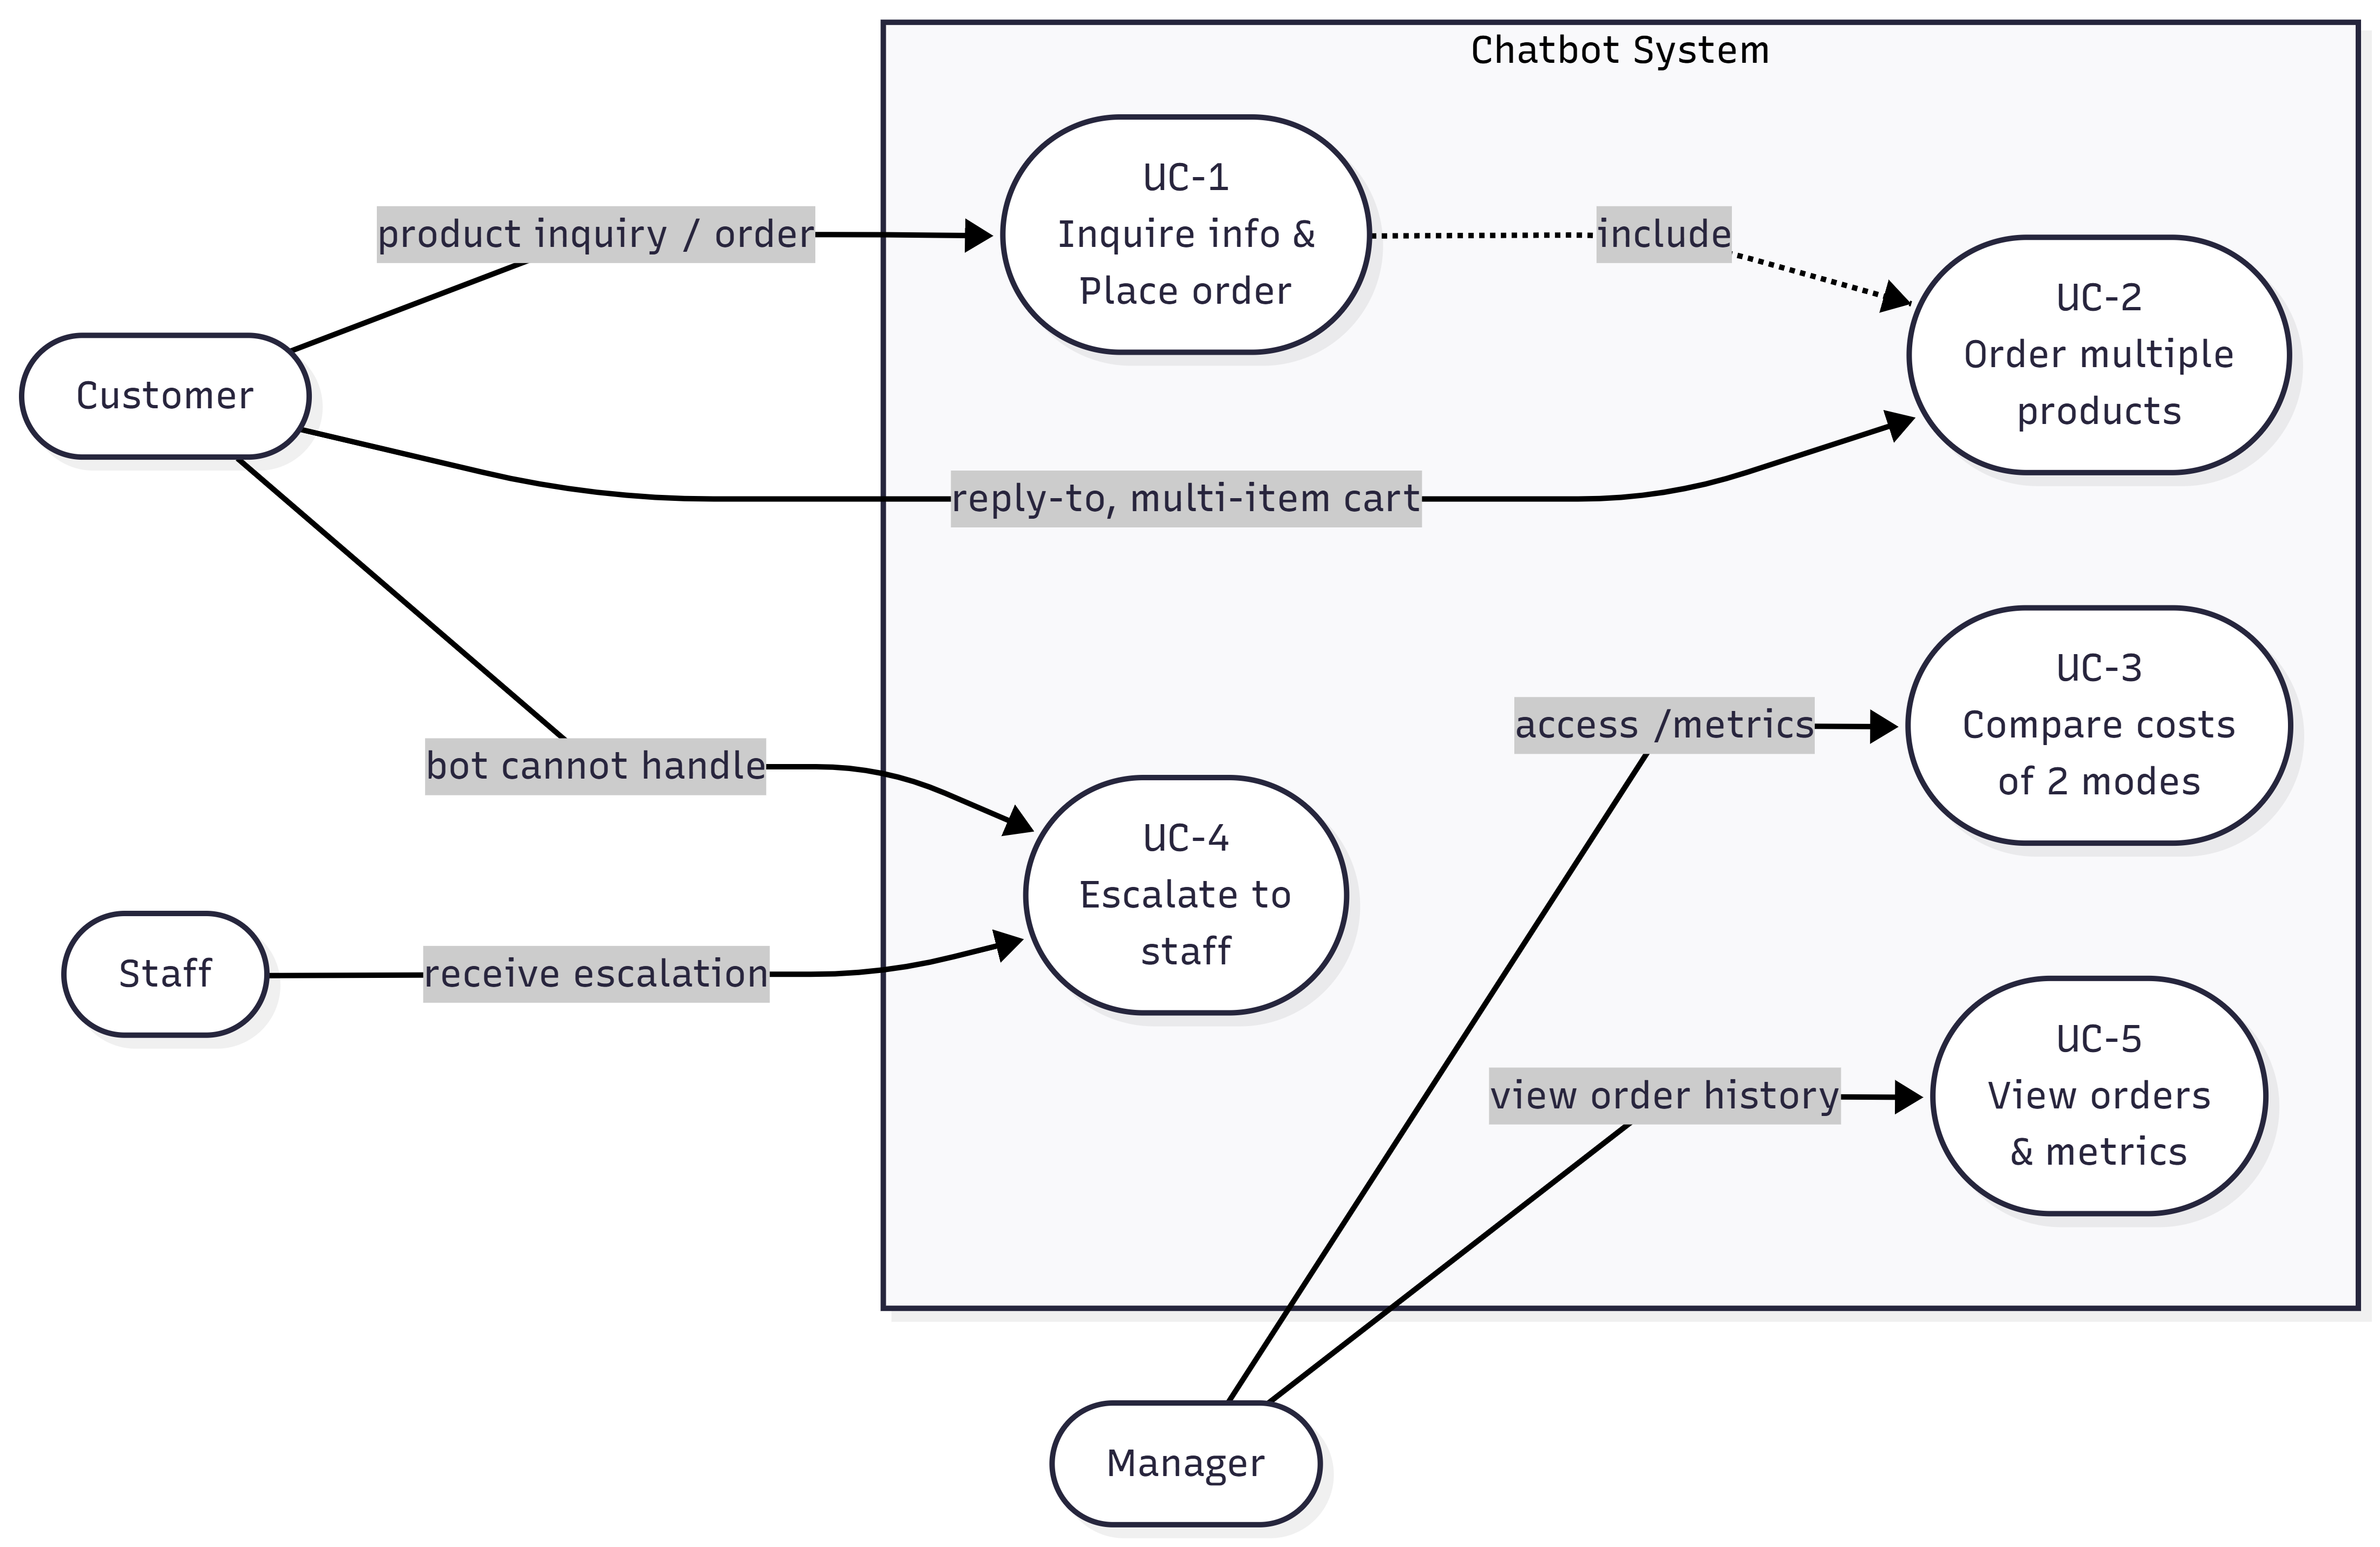
\includegraphics[width=0.92\linewidth]{Usecase.png}
\caption{Use Case Diagram --- Hệ thống Chatbot LEGO}
\label{fig:usecases}
\end{figure}

\begin{table}[H]
\centering
\caption{Mô tả các Use Case chính}
\label{tab:usecases}
\begin{tabularx}{\linewidth}{llX}
\toprule
\textbf{ID} & \textbf{Tên} & \textbf{Mô tả ngắn} \\
\midrule
UC-1 & Hỏi thông tin \& đặt hàng
  & Khách hỏi sản phẩm $\rightarrow$ bot đề xuất top-3
    $\rightarrow$ khách xác nhận $\rightarrow$ điền thông tin
    $\rightarrow$ xác nhận thanh toán $\rightarrow$ ghi đơn. \\
UC-2 & Đặt nhiều sản phẩm
  & Khách reply-to nhiều tin nhắn để chọn từng sản phẩm;
    giỏ hàng tích luỹ nhiều món trước khi chốt. \\
UC-3 & So sánh chi phí 2 chế độ
  & Quản lý xem trang \texttt{/metrics}: latency, token,
    chi phí ước tính giữa chế độ hybrid và full-LLM. \\
UC-4 & Escalate sang nhân viên
  & Bot không xử lý được 5 lượt liên tiếp (nhánh J)
    $\rightarrow$ chuyển sang nhân viên kèm toàn bộ context. \\
UC-5 & Xem đơn hàng \& metrics
  & Quản lý xem lịch sử đơn hàng trong SQLite và log JSONL. \\
\bottomrule
\end{tabularx}
\end{table}

\subsection{Chi tiết UC-1: Hỏi thông tin và đặt hàng}

\textbf{Tiền điều kiện:} Khách mở giao diện chat. \\
\textbf{Luồng chính:}
\begin{enumerate}
  \item Khách gõ: ``còn con Ferrari không shop?''
  \item Bot phân loại intent (\texttt{ask\_product\_availability}),
        NER trích \texttt{PRODUCT\_NAME = ``Ferrari''};
        matcher trả top-3 từ catalog 11.362 sản phẩm.
  \item Khách chọn: ``số 1''; bot xác nhận và hỏi thông tin giao hàng.
  \item Khách cung cấp \texttt{NAME}, \texttt{PHONE}, \texttt{ADDRESS};
        bot điền slot và hỏi phương thức thanh toán.
  \item Khách chọn \texttt{COD}/\texttt{chuyển khoản};
        đơn được ghi SQLite, bot gửi tóm tắt.
\end{enumerate}
\textbf{Luồng thay thế:}
Nếu khách cung cấp ngân sách, matcher lọc theo
\texttt{MIN\_BUDGET}--\texttt{MAX\_BUDGET} trước khi cosine search.

% ============================================================
%  CHƯƠNG 7 — KẾT QUẢ VÀ ĐÁNH GIÁ
% ============================================================
\chapter{Kết quả Tổng hợp và Đánh giá Hệ thống}

\section{So sánh Hybrid vs Full-LLM}

\begin{table}[H]
\centering
\caption{So sánh định lượng hai chế độ chatbot}
\label{tab:compare_modes}
\begin{tabular}{lcc}
\toprule
\textbf{Chỉ số} & \textbf{Hybrid (NLU + rule-based)} & \textbf{Full-LLM} \\
\midrule
Latency trung bình     & $\approx 150$--$300$\,ms & $\approx 1{,}5$--$4$\,s \\
LLM token/lượt         & 0                        & $\approx 600$--$1.300$ \\
Chi phí/1.000 lượt     & $\approx 0$\,đồng        & $\approx 6.000$--$15.000$\,đồng \\
Chi phí/10.000 lượt    & $\approx 0$\,đồng        & $\approx 60.000$--$150.000$\,đồng \\
Kiểm soát hành vi      & Cao (rule xác định)      & Thấp (LLM tự quyết) \\
Xử lý luồng đặt hàng  & Theo state machine       & Theo ngữ cảnh LLM \\
Cập nhật nghiệp vụ     & Sửa rule/template        & Sửa prompt \\
\bottomrule
\end{tabular}
\end{table}

\textbf{Phân tích chi phí theo lưu lượng:}
Với 1.000 lượt chat/tháng (cửa hàng nhỏ), chi phí full-LLM
ước tính 60.000--150.000 VNĐ/tháng — có thể chấp nhận được.
Tuy nhiên, với 10.000+ lượt/tháng, con số này trở nên đáng kể
và hệ thống hybrid tỏ ra vượt trội về mặt kinh tế.

\section{Đánh giá định tính qua log hội thoại}

\subsection{Kịch bản end-to-end điển hình}

Bảng sau minh họa một hội thoại đặt hàng hoàn chỉnh
qua hệ thống hybrid:

\begin{table}[H]
\centering
\caption{Ví dụ hội thoại end-to-end qua hệ thống Hybrid}
\label{tab:convo_example}
\begin{tabularx}{\linewidth}{lXl}
\toprule
\textbf{Lượt} & \textbf{Nội dung} & \textbf{Nhánh} \\
\midrule
Khách & ``shop ơi còn con ferrari k ạ'' & E \\
Bot   & ``Dạ có 3 mẫu Ferrari: (1) F40 — 1.378.000đ, (2) SF-24 F1...'' & — \\
Khách & ``lấy số 1 đi'' & D \\
Bot   & ``Dạ bạn muốn thêm Ferrari F40 vào giỏ không ạ?'' & — \\
Khách & ``ừ'' & A.1 \\
Bot   & ``Đã thêm Ferrari F40. Bạn muốn đặt hàng luôn không?'' & — \\
Khách & ``ok đặt luôn'' & F / B \\
Bot   & ``Bạn cho shop xin tên, SĐT và địa chỉ nhé ạ'' & — \\
Khách & ``Nguyễn An, 0912345678, 30 Cát Linh Hà Nội'' & B / I \\
Bot   & ``Dạ xác nhận đơn: 1 × Ferrari F40, 1.378.000đ...'' & — \\
Khách & ``ck nha'' & B \\
Bot   & ``Shop gửi STK: ... Bạn chuyển khoản xong gửi bill nhé!'' & — \\
\bottomrule
\end{tabularx}
\end{table}

\subsection{Phân tích ổn định hệ thống}

Trong quá trình kiểm thử thực tế (log ngày 2026-06-16),
4 loại lỗi đã được phát hiện và sửa chữa:

\begin{enumerate}
  \item \textbf{Stage=done loop:} Hệ thống tiếp tục xử lý intent
        sau khi đơn đã hoàn tất — đã thêm nhánh A.0-done.
  \item \textbf{QUANTITY tại await\_confirm:} Cập nhật số lượng
        không trigger lại tóm tắt đơn — đã sửa nhánh B.
  \item \textbf{``oke'' fallback:} Câu chấp thuận thông thường
        không được nhận diện là affirm — đã mở rộng hàm \texttt{\_affirmative()}.
  \item \textbf{Auto-add từ suggest flow:} Chọn số từ danh sách gợi ý
        bị thêm thẳng vào giỏ mà không qua xác nhận —
        đã thêm action \texttt{suggest\_confirm}.
\end{enumerate}

\section{Thảo luận: Khi nào dùng Hybrid, khi nào Full-LLM}

\begin{itemize}
  \item \textbf{Hybrid phù hợp} khi: cần kiểm soát chặt chẽ luồng nghiệp vụ,
        lưu lượng cao, ngân sách vận hành hạn chế, hoặc khi các kịch bản
        hội thoại có thể được mô tả đầy đủ bằng rule.
  \item \textbf{Full-LLM phù hợp} khi: kịch bản đa dạng khó đoán trước,
        cần ngôn ngữ phong phú và linh hoạt, hoặc trong giai đoạn
        khởi động khi chưa có đủ dữ liệu để fine-tune mô hình NLU.
\end{itemize}

% ============================================================
%  KẾT LUẬN
% ============================================================
\chapter*{Kết luận và Hướng phát triển}
\addcontentsline{toc}{chapter}{Kết luận và Hướng phát triển}

\section*{Tổng kết kết quả}

Đề tài đã trả lời được ba câu hỏi nghiên cứu đặt ra:

\begin{enumerate}
  \item \textbf{Câu hỏi 1:} Hệ thống hybrid NLU + rule-based
        đủ khả năng xử lý hội thoại bán hàng thực tế.
        Mô hình phân loại intent đạt Macro-F1 = 0,9022 trên tập test,
        và hệ thống hoàn thành được luồng đặt hàng end-to-end.
  \item \textbf{Câu hỏi 2:} Chi phí vận hành chênh lệch đáng kể:
        hệ thống hybrid có chi phí API gần bằng 0, trong khi full-LLM
        tiêu thụ 600--1.300 token/lượt, tương đương 6--15 VNĐ/lượt
        (khoảng 6.000--15.000 VNĐ/1.000 lượt). Latency của hybrid
        thấp hơn 5--20 lần so với full-LLM.
  \item \textbf{Câu hỏi 3:} Chuẩn hóa văn bản + phân đoạn từ giúp
        PhoBERT vượt ViSoBERT trên tác vụ phân loại intent (sentence-level),
        xác nhận giả thuyết rằng preprocessing tường minh có thể bù đắp
        cho register mismatch.
\end{enumerate}

\section*{Hạn chế}

\begin{itemize}
  \item NER Micro-F1 $\approx 0,70$ vẫn còn chỗ cải thiện,
        đặc biệt với \texttt{ADDRESS} và các nhãn hiếm.
  \item Từ điển chuẩn hóa teen-code cần được bổ sung liên tục.
  \item Dữ liệu huấn luyện được thu thập từ một cửa hàng duy nhất;
        khả năng tổng quát sang miền khác cần kiểm chứng thêm.
\end{itemize}

\section*{Hướng phát triển}

\begin{itemize}
  \item \textbf{Tăng dữ liệu NER:} Thu thập thêm mẫu cho nhãn hiếm,
        áp dụng active learning để chọn mẫu gán nhãn hiệu quả.
  \item \textbf{Chuẩn hóa thần kinh:} Nghiên cứu seq2seq normalization
        khi có đủ corpus song song (informal $\rightarrow$ formal).
  \item \textbf{Tích hợp đa kênh:} Mở rộng sang Zalo và Facebook Messenger API.
  \item \textbf{Đánh giá người dùng thực:} Thu thập phản hồi
        từ nhân viên cửa hàng để đánh giá chất lượng hội thoại.
\end{itemize}

% ============================================================
%  TÀI LIỆU THAM KHẢO
% ============================================================
\begin{thebibliography}{99}
\addcontentsline{toc}{chapter}{Tài liệu tham khảo}

\bibitem{devlin2019bert}
J. Devlin, M.-W. Chang, K. Lee, và K. Toutanova,
``BERT: Pre-training of Deep Bidirectional Transformers for Language Understanding,''
trong \textit{Proc. NAACL-HLT}, Minneapolis, MN, USA, 2019, tr. 4171--4186.

\bibitem{vaswani2017attention}
A. Vaswani, N. Shazeer, N. Parmar, J. Uszkoreit, L. Jones, A. N. Gomez,
Ł. Kaiser, và I. Polosukhin,
``Attention Is All You Need,''
trong \textit{Proc. NeurIPS}, Long Beach, CA, USA, 2017, tr. 5998--6008.

\bibitem{nguyen2020phobert}
D. Q. Nguyen và A. T. Nguyen,
``PhoBERT: Pre-trained Language Models for Vietnamese,''
trong \textit{Findings of EMNLP}, Online, 2020, tr. 1037--1042.

\bibitem{visobert2023}
T.-L. Nguyen, V.-N. Tran, V.-D. Ngo, T.-H. Nguyen, T.-T. Tran, và T.-S. Le,
``ViSoBERT: A Pre-Trained Language Model for Vietnamese Social Media Text Processing,''
trong \textit{Proc. EMNLP}, Singapore, 2023, tr. 12102--12118.

\bibitem{conneau2020xlmr}
A. Conneau, K. Khandelwal, N. Goyal, V. Chaudhary, G. Wenzek, F. Guzmán,
E. Grave, M. Ott, L. Zettlemoyer, và V. Stoyanov,
``Unsupervised Cross-lingual Representation Learning at Scale,''
trong \textit{Proc. ACL}, Online, 2020, tr. 8440--8451.

\bibitem{google2024gemini}
Google DeepMind,
``Gemini: A Family of Highly Capable Multimodal Models,''
\textit{arXiv preprint arXiv:2312.11805}, 2024.

\bibitem{lewis2020rag}
P. Lewis, E. Perez, A. Piktus, F. Petroni, V. Karpukhin, N. Goyal,
H. Küttler, M. Lewis, W.-T. Yih, T. Rocktäschel, S. Riedel, và D. Kiela,
``Retrieval-Augmented Generation for Knowledge-Intensive NLP Tasks,''
trong \textit{Proc. NeurIPS}, Online, 2020, tr. 9459--9474.

\bibitem{underthesea}
V. Anh,
``underthesea: Vietnamese NLP Toolkit,''
GitHub repository, 2021.
[Online]. Available: \url{https://github.com/undertheseanlp/underthesea}

\bibitem{sechidis2011stratification}
K. Sechidis, G. Tsoumakas, và I. Vlahavas,
``On the Stratification of Multi-Label Data,''
trong \textit{Proc. ECML PKDD}, Athens, Greece, 2011, tr. 145--158.

\bibitem{rapidfuzz}
M. Bachmann,
``RapidFuzz: A fast string matching library for Python,''
GitHub repository, 2021.
[Online]. Available: \url{https://github.com/rapidfuzz/RapidFuzz}

\bibitem{liu2019roberta}
Y. Liu, M. Ott, N. Goyal, J. Du, M. Joshi, D. Chen, O. Levy,
M. Lewis, L. Zettlemoyer, và V. Stoyanov,
``RoBERTa: A Robustly Optimized BERT Pretraining Approach,''
\textit{arXiv preprint arXiv:1907.11692}, 2019.

\bibitem{lample2016ner}
G. Lample, M. Ballesteros, S. Subramanian, K. Kawakami, và C. Dyer,
``Neural Architectures for Named Entity Recognition,''
trong \textit{Proc. NAACL-HLT}, San Diego, CA, USA, 2016, tr. 260--270.

\bibitem{doccano2018}
H. Nakayama, T. Kubo, J. Kamura, Y. Taniguchi, và X. Liang,
``doccano: Text Annotation Tool for Human,''
GitHub repository, 2018.
[Online]. Available: \url{https://github.com/doccano/doccano}

\bibitem{rebrickable}
Rebrickable,
``Rebrickable API --- LEGO Set Database,''
[Online]. Available: \url{https://rebrickable.com/api/}
[Accessed: \placeholder{tháng/năm truy cập}]

\end{thebibliography}

% ============================================================
%  PHỤ LỤC
% ============================================================
\appendix

\chapter{Danh sách đầy đủ 32 lớp Intent}
\label{app:intents}

\begin{longtable}{lX}
\caption{32 lớp intent và mô tả} \label{tab:all_intents} \\
\toprule
\textbf{Intent} & \textbf{Ví dụ câu} \\
\midrule
\endfirsthead
\multicolumn{2}{c}{\textit{(tiếp theo)}} \\
\toprule \textbf{Intent} & \textbf{Ví dụ câu} \\ \midrule
\endhead
\bottomrule \endlastfoot
\texttt{Greeting}                    & ``shop ơi'', ``chào shop'' \\
\texttt{Goodbye}                     & ``cảm ơn shop nhé'', ``thôi thôi'' \\
\texttt{give\_product}               & ``mình muốn đặt con ferrari'' \\
\texttt{add\_product}                & ``thêm cái đó vào giỏ hộ mình'' \\
\texttt{agree\_order}                & ``ok đặt luôn đi'', ``chốt nha'' \\
\texttt{customer\_reject}            & ``thôi không lấy nữa'', ``bỏ đi'' \\
\texttt{ask\_product\_info}          & ``bộ này có bao nhiêu mảnh ạ?'' \\
\texttt{ask\_product\_availability}  & ``còn hàng không shop?'' \\
\texttt{ask\_product\_suggestion}    & ``shop gợi ý cho mình bộ nào với'' \\
\texttt{ask\_product\_image}         & ``shop gửi hình đi'' \\
\texttt{ask\_legit}                  & ``hàng chính hãng không shop?'' \\
\texttt{ask\_payment\_method}        & ``thanh toán thế nào ạ?'' \\
\texttt{ask\_shipping\_fee}          & ``ship hà nội bao nhiêu?'' \\
\texttt{ask\_delivery\_time}         & ``bao lâu nhận được?'' \\
\texttt{ask\_order\_status}          & ``đơn mình tới đâu rồi shop?'' \\
\texttt{ask\_order\_wait\_time}      & ``còn bao lâu nữa mới giao?'' \\
\texttt{ask\_shop\_info}             & ``shop ở đâu vậy?'' \\
\texttt{ask\_find\_product}          & ``shop tìm giúp mình bộ X'' \\
\texttt{provide\_cus\_inf}           & ``mình tên An, SĐT 0912...'' \\
\texttt{ask\_gift\_wrap}             & ``shop gói quà được không?'' \\
\texttt{ask\_gift\_suggestion}       & ``mua quà sinh nhật cho bé 6 tuổi'' \\
\texttt{ask\_budget}                 & ``tầm 500k có gì không shop?'' \\
\texttt{ask\_product\_price}         & ``bộ này giá bao nhiêu?'' \\
\texttt{ask\_promotion}              & ``có khuyến mãi không shop?'' \\
\texttt{complain}                    & ``hàng bị lỗi rồi shop ơi'' \\
\texttt{thanks}                      & ``cảm ơn shop nhiều nhé'' \\
\texttt{other}                       & Câu ngoài phạm vi chatbot \\
\textit{... (5 lớp còn lại)}         & \placeholder{bổ sung} \\
\end{longtable}

\chapter{Cấu trúc thư mục dự án}
\label{app:structure}

\begin{lstlisting}
GraduateProject/
├── approach1/              SVM + TF-IDF notebooks
├── approach2/              ViSoBERT intent notebook
├── approach3/              PhoBERT + normalize (training)
├── approach3_results/      Checkpoint đã train
│   ├── results/
│   │   ├── intent_model/   PhoBERT checkpoint
│   │   ├── mlb.joblib      MultiLabelBinarizer (32 classes)
│   │   └── metrics.json    Per-class thresholds
├── approach4/              XLM-RoBERTa notebook
├── ner/
│   ├── ner_visobertv2.ipynb    NER training (được chọn)
│   └── results/ner_model/      ViSoBERT NER checkpoint
├── final_data/
│   └── products_2010_2026_updated.json
├── chatbot/
│   ├── app.py              FastAPI server
│   ├── pipeline.py         14-branch pipeline
│   ├── nlu.py              PhoBERT + ViSoBERT loader
│   ├── state.py            SessionState + SlotStore
│   ├── reply.py            Template reply
│   ├── rag.py              Hybrid RAG
│   ├── llm_baseline.py     Gemini + RAG + logging
│   ├── logger.py           TurnLogger (JSONL)
│   └── db.py               SQLite
└── logs/                   chat_YYYYMMDD.jsonl
\end{lstlisting}

\end{document}
